% !TEX program = xelatex
% Compile: xelatex → bibtex → xelatex → xelatex
\documentclass[12pt,a4paper]{article}

\usepackage{fontspec}
\usepackage[english]{babel}
\usepackage[backend=bibtex,style=authoryear,sorting=nyt,maxcitenames=2]{biblatex}
\addbibresource{references.bib}
\usepackage{amsmath,amssymb}
\usepackage{graphicx}
\usepackage{booktabs}
\usepackage{hyperref}
\hypersetup{
    colorlinks=true,
    linkcolor=blue,
    citecolor=blue,
    urlcolor=blue
}
\usepackage[margin=2.5cm]{geometry}
\usepackage{subcaption}
\usepackage{xcolor}
\usepackage{siunitx}

\title{\textbf{Endogenous Technology and Network Dynamics in AI Adoption:\\
A Factorial Agent-Based Study}}

\author{Mateusz Maciaszek}

\date{{\small February 2026}}

\begin{document}

\maketitle

%----------------------------------------------------------------------
\begin{abstract}
%----------------------------------------------------------------------

Papers I--IV of this series established that the automation transition in a
stock-flow consistent agent-based model (SFC-ABM) exhibits a reentrant phase
transition at a critical basic disposable payment $\mathrm{BDP}_c = 500$~PLN,
with mean-field universality ($\gamma \approx 1.0$) that is invariant to
network topology and decision-rule specification. However, both the sectoral
elasticity of substitution~$\sigma$ and the inter-firm network were held
\emph{exogenous and static}. This paper tests whether universality survives
endogenization through a $2 \times 2$ factorial design: (fixed/endogenous
$\sigma$) $\times$ (static/dynamic network). Endogenous~$\sigma$ follows an
Arthur-style increasing-returns learning rule; dynamic networks implement
death--birth with preferential rewiring. Across 10,080 Monte Carlo simulations
(4 factorial cells + 2 marginal sweeps, 21 BDP levels, 30 seeds each), we
find that: (i)~the reentrant adoption shape survives in all four cells;
(ii)~endogenous~$\sigma$ alone preserves $\mathrm{BDP}_c = 500$~PLN up to
moderate learning rates ($\lambda \le 0.02$); (iii)~dynamic rewiring shifts
the critical point to $\mathrm{BDP}_c = 750$ for intermediate rates
$\rho \in [0.02, 0.10]$, but the shift reverses at high~$\rho$;
(iv)~the combined effect is superadditive (+6.5~pp peak adoption vs.\
baseline); and (v)~endogenous~$\sigma$ does not produce self-organized
criticality---instead, a positive feedback loop links adoption and technology
growth. The principal finding is that endogenization perturbs but does not
destroy the phase structure: $\mathrm{BDP}_c$ shifts by at most one grid
spacing (250~PLN), and the reentrant shape---the key policy-relevant
feature---is fully robust.

\medskip\noindent
\textbf{Keywords:} agent-based model, stock-flow consistency, automation,
universal basic income, endogenous technology, dynamic networks,
phase transition, self-organized criticality

\medskip\noindent
\textbf{JEL codes:} C63, E17, J24, O33

\medskip\noindent
\textbf{Code \& Data:}
\url{https://github.com/mmaciaszek/complexity-econ}

\end{abstract}

\newpage
\tableofcontents
\newpage


%======================================================================
\section{Introduction}\label{sec:intro}
%======================================================================

The preceding four papers in this series constructed a stock-flow consistent
agent-based model (SFC-ABM) of AI-driven automation and used it to
characterize the macroeconomic response to a universal basic disposable
payment (BDP). Paper~I \parencite{Maciaszek2026a} identified the
\emph{acceleration paradox}: moderate BDP amplifies rather than cushions
labor market disruption, producing bimodal adoption outcomes at
$\mathrm{BDP} = 2{,}000$~PLN. Paper~II \parencite{Maciaszek2026b}
showed that the monetary regime matters more than the subsidy level---the
PLN float permits a reentrant (inverted-U) adoption curve, while EUR with
Stability and Growth Pact constraints creates a closed island in
$(\mathrm{BDP}, \sigma)$ space. Paper~III \parencite{Maciaszek2026c}
estimated sectoral elasticities of substitution $\sigma_s$ empirically
using GMM and Bayesian methods, finding that $\sigma$ calibration barely
affects the critical point ($\Delta\sigma$ of 5--9$\times$ $\Rightarrow$
$\Delta$adoption of 1.5~pp). Paper~IV \parencite{Maciaszek2026d}
mapped the full phase diagram, demonstrating topology universality
($\mathrm{BDP}_c = 500$ across WS, ER, BA, and lattice networks),
mean-field critical exponents ($\gamma \approx 1.0$), and decision-rule
invariance.

A striking limitation of these results is that both the technology parameter
$\sigma_s$ and the network of inter-firm influences are \emph{exogenous and
static}. In reality, technology evolves endogenously through learning-by-doing
\parencite{Arrow1962}, increasing returns \parencite{Arthur1989,Arthur1994},
and path dependence \parencite{David1985}. Firm networks also evolve:
bankrupt firms exit, new entrants form connections, and successful adopters
attract imitators \parencite{Jackson2002, Battiston2012}. The question is
whether the universality established in Paper~IV---a property of the static,
exogenous model---survives when these mechanisms are activated.

This question connects to the concept of \emph{self-organized criticality}
(SOC), introduced by \textcite{Bak1987} and elaborated in \textcite{Bak1996}.
In SOC systems, the dynamics drive the system toward the critical point
without external tuning. If endogenous $\sigma$ evolution causes the
technology parameter to converge to a value near the phase boundary,
the system could exhibit SOC---a qualitatively different regime from
the externally tuned transitions studied in Papers~I--IV.

We address these questions through a $2 \times 2$ factorial experimental
design, crossing endogenous vs.\ static $\sigma$ with dynamic vs.\ static
network topology. This yields four cells---a baseline replicating Paper~IV,
two single-mechanism treatments, and a full endogenous cell---each swept
across 21 BDP levels with 30 Monte Carlo seeds. Two additional marginal
sensitivity campaigns isolate the effects of the learning rate~$\lambda$
and the rewiring rate~$\rho$. The total experimental budget is 10,080
simulations.


%======================================================================
\section{Model Extensions}\label{sec:model}
%======================================================================

We extend the SFC-ABM engine described in Papers~I--IV with two new
mechanisms, each controlled by a single parameter that defaults to zero
(recovering the baseline model).

%----------------------------------------------------------------------
\subsection{Endogenous $\sigma$ via Learning-by-Doing}\label{sec:sigma}
%----------------------------------------------------------------------

The elasticity of substitution $\sigma_s$ governs the profitability
threshold for automation adoption in sector~$s$
\parencite[see][]{Maciaszek2026a}:
\begin{equation}\label{eq:threshold}
  \theta_s = \min\!\bigl(1.0,\; 0.88 + 0.075 \cdot
  \log_{10}(\sigma_s)\bigr).
\end{equation}

In Papers~I--IV, $\sigma_s$ was fixed at its calibrated value throughout
the simulation. We now allow $\sigma_s$ to evolve endogenously following
an Arthur-style increasing-returns rule
\parencite{Arthur1989,Arrow1962}:
\begin{equation}\label{eq:sigma_dynamics}
  \sigma_s(t+1) = \sigma_s(t) + \lambda \cdot \sigma_s(t) \cdot
  \phi_s(t) \cdot \left(1 - \frac{\sigma_s(t)}{C_s}\right),
\end{equation}
where $\phi_s(t)$ is the adoption rate in sector~$s$ at time~$t$,
$\lambda \ge 0$ is the \emph{learning rate}, and $C_s = \sigma_s^{(0)}
\cdot c$ is a logistic cap ($c = 3$ by default, so each sector's
$\sigma$ can at most triple). The logistic term prevents unbounded growth.
A \emph{ratchet constraint} ensures $\sigma$ never decreases:
$\sigma_s(t+1) \ge \sigma_s(t)$. When $\lambda = 0$, the update is a
no-op and the model reduces to the Paper~IV baseline.

The economic interpretation is learning-by-doing: sectors with higher
adoption rates accumulate experience that raises the effective
substitutability between labor and AI capital. The ratchet embodies
irreversibility of technological knowledge---once learned, techniques
are not forgotten.

%----------------------------------------------------------------------
\subsection{Dynamic Network with Death--Birth Rewiring}\label{sec:network}
%----------------------------------------------------------------------

In the baseline model, firms interact on a Watts--Strogatz small-world
network ($k = 6$, $p = 0.10$) that remains fixed for the entire 120-month
simulation \parencite{Watts1998}. We now introduce dynamic rewiring:
each month, with probability~$\rho$ per bankrupt firm, the following
occurs:
\begin{enumerate}
  \item \textbf{Death}: the bankrupt firm's edges are removed from
  the adjacency list.
  \item \textbf{Birth}: a new Traditional-technology firm replaces the
  bankrupt slot.
  \item \textbf{Preferential attachment}: the new firm forms~$k$
  connections to surviving firms, with probability proportional to each
  survivor's current degree \parencite{Barabasi1999}.
\end{enumerate}

This creates endogenous degree heterogeneity: successful firms (which
tend to survive) accumulate connections over time, while new entrants
start with exactly $k$~links. When $\rho = 0$, no rewiring occurs and
the model reduces to the static baseline. The mechanism is motivated by
the empirical observation that inter-firm networks restructure around
surviving hubs during economic transitions \parencite{Battiston2012,
Jackson2002}.

%----------------------------------------------------------------------
\subsection{Parameter Configuration}\label{sec:params}
%----------------------------------------------------------------------

The two new parameters are passed via environment variables, following
the convention established in Paper~IV:

\begin{table}[htbp]
\centering
\small
\caption{New parameters introduced in Paper~V.}\label{tab:params}
\begin{tabular}{llll}
\toprule
\textbf{Parameter} & \textbf{Env var} & \textbf{Default} & \textbf{Interpretation} \\
\midrule
$\lambda$ & \texttt{SIGMA\_LAMBDA} & 0.0 & Learning rate (endogenous $\sigma$) \\
$c$ & \texttt{SIGMA\_CAP\_MULT} & 3.0 & Logistic cap multiplier \\
$\rho$ & \texttt{REWIRE\_RHO} & 0.0 & Rewiring probability \\
\bottomrule
\end{tabular}
\end{table}

All other model parameters are unchanged from Paper~IV. The simulation
runs 10,000 firms across 6 sectors for 120 months with an automation
shock at month~30, under the PLN monetary regime.


%======================================================================
\section{Experimental Design}\label{sec:method}
%======================================================================

%----------------------------------------------------------------------
\subsection{Factorial Core (C1)}\label{sec:c1}
%----------------------------------------------------------------------

The primary experiment is a $2 \times 2$ factorial design crossing
endogenous $\sigma$ ($\lambda \in \{0, 0.02\}$) with dynamic network
topology ($\rho \in \{0, 0.1\}$):

\begin{table}[htbp]
\centering
\small
\caption{$2 \times 2$ factorial design.}\label{tab:factorial}
\begin{tabular}{lcccc}
\toprule
& & \multicolumn{2}{c}{\textbf{Network}} \\
\cmidrule(lr){3-4}
& & Static ($\rho=0$) & Dynamic ($\rho=0.1$) \\
\midrule
\multirow{2}{*}{\textbf{$\sigma$}}
  & Fixed ($\lambda=0$) & Cell A: baseline & Cell C: network-only \\
  & Endo ($\lambda=0.02$) & Cell B: $\sigma$-only & Cell D: full endogenous \\
\bottomrule
\end{tabular}
\end{table}

Each cell is swept across 21 BDP levels (0, 250, 500, \ldots, 5{,}000~PLN)
with 30 Monte Carlo seeds per level, yielding $4 \times 21 \times 30 =
2{,}520$ simulations.

%----------------------------------------------------------------------
\subsection{Marginal Sensitivity Sweeps}\label{sec:c2c3}
%----------------------------------------------------------------------

To isolate marginal effects, we run two additional campaigns:

\textbf{C2: Learning rate sensitivity.} Fixed $\rho = 0$ (static network),
$\lambda \in \{0, 0.005, 0.01, 0.02, 0.05, 0.1\}$. Total:
$6 \times 21 \times 30 = 3{,}780$ simulations.

\textbf{C3: Rewiring rate sensitivity.} Fixed $\lambda = 0$ (static
$\sigma$), $\rho \in \{0, 0.02, 0.05, 0.1, 0.2, 0.5\}$. Total:
$6 \times 21 \times 30 = 3{,}780$ simulations.

\textbf{Grand total:} $2{,}520 + 3{,}780 + 3{,}780 = \mathbf{10{,}080}$
Monte Carlo simulations (comparable to Paper~IV's 18,540).

%----------------------------------------------------------------------
\subsection{Identification Strategy}\label{sec:identification}
%----------------------------------------------------------------------

We identify the critical BDP as the argmax of the adoption variance
across seeds:
\begin{equation}\label{eq:bdpc}
  \mathrm{BDP}_c = \arg\max_{\mathrm{BDP}} \;
  \mathrm{Var}\!\bigl[\phi(\mathrm{BDP})\bigr],
\end{equation}
where $\phi(\mathrm{BDP})$ is the terminal adoption rate across
30 seeds at a given BDP level. This variance-peak method serves as
a susceptibility proxy, following the approach established in
Paper~IV \parencite[see][]{Maciaszek2026d, Stanley1971, Binder2010}.


%======================================================================
\section{Results}\label{sec:results}
%======================================================================

%----------------------------------------------------------------------
\subsection{Factorial Comparison: Adoption Curves}\label{sec:bifurcation}
%----------------------------------------------------------------------

Figure~\ref{fig:bifurcation} displays the adoption--BDP bifurcation
diagram for all four factorial cells. The central finding is that the
\emph{reentrant shape} (inverted-U)---the key policy-relevant feature
established in Papers~I--II---survives in all four cells. Peak adoption
occurs at low BDP (250~PLN) in each case, followed by a monotonic decline
as rising inflation triggers central bank rate hikes that increase
automation CAPEX costs.

\begin{figure}[htbp]
    \centering
    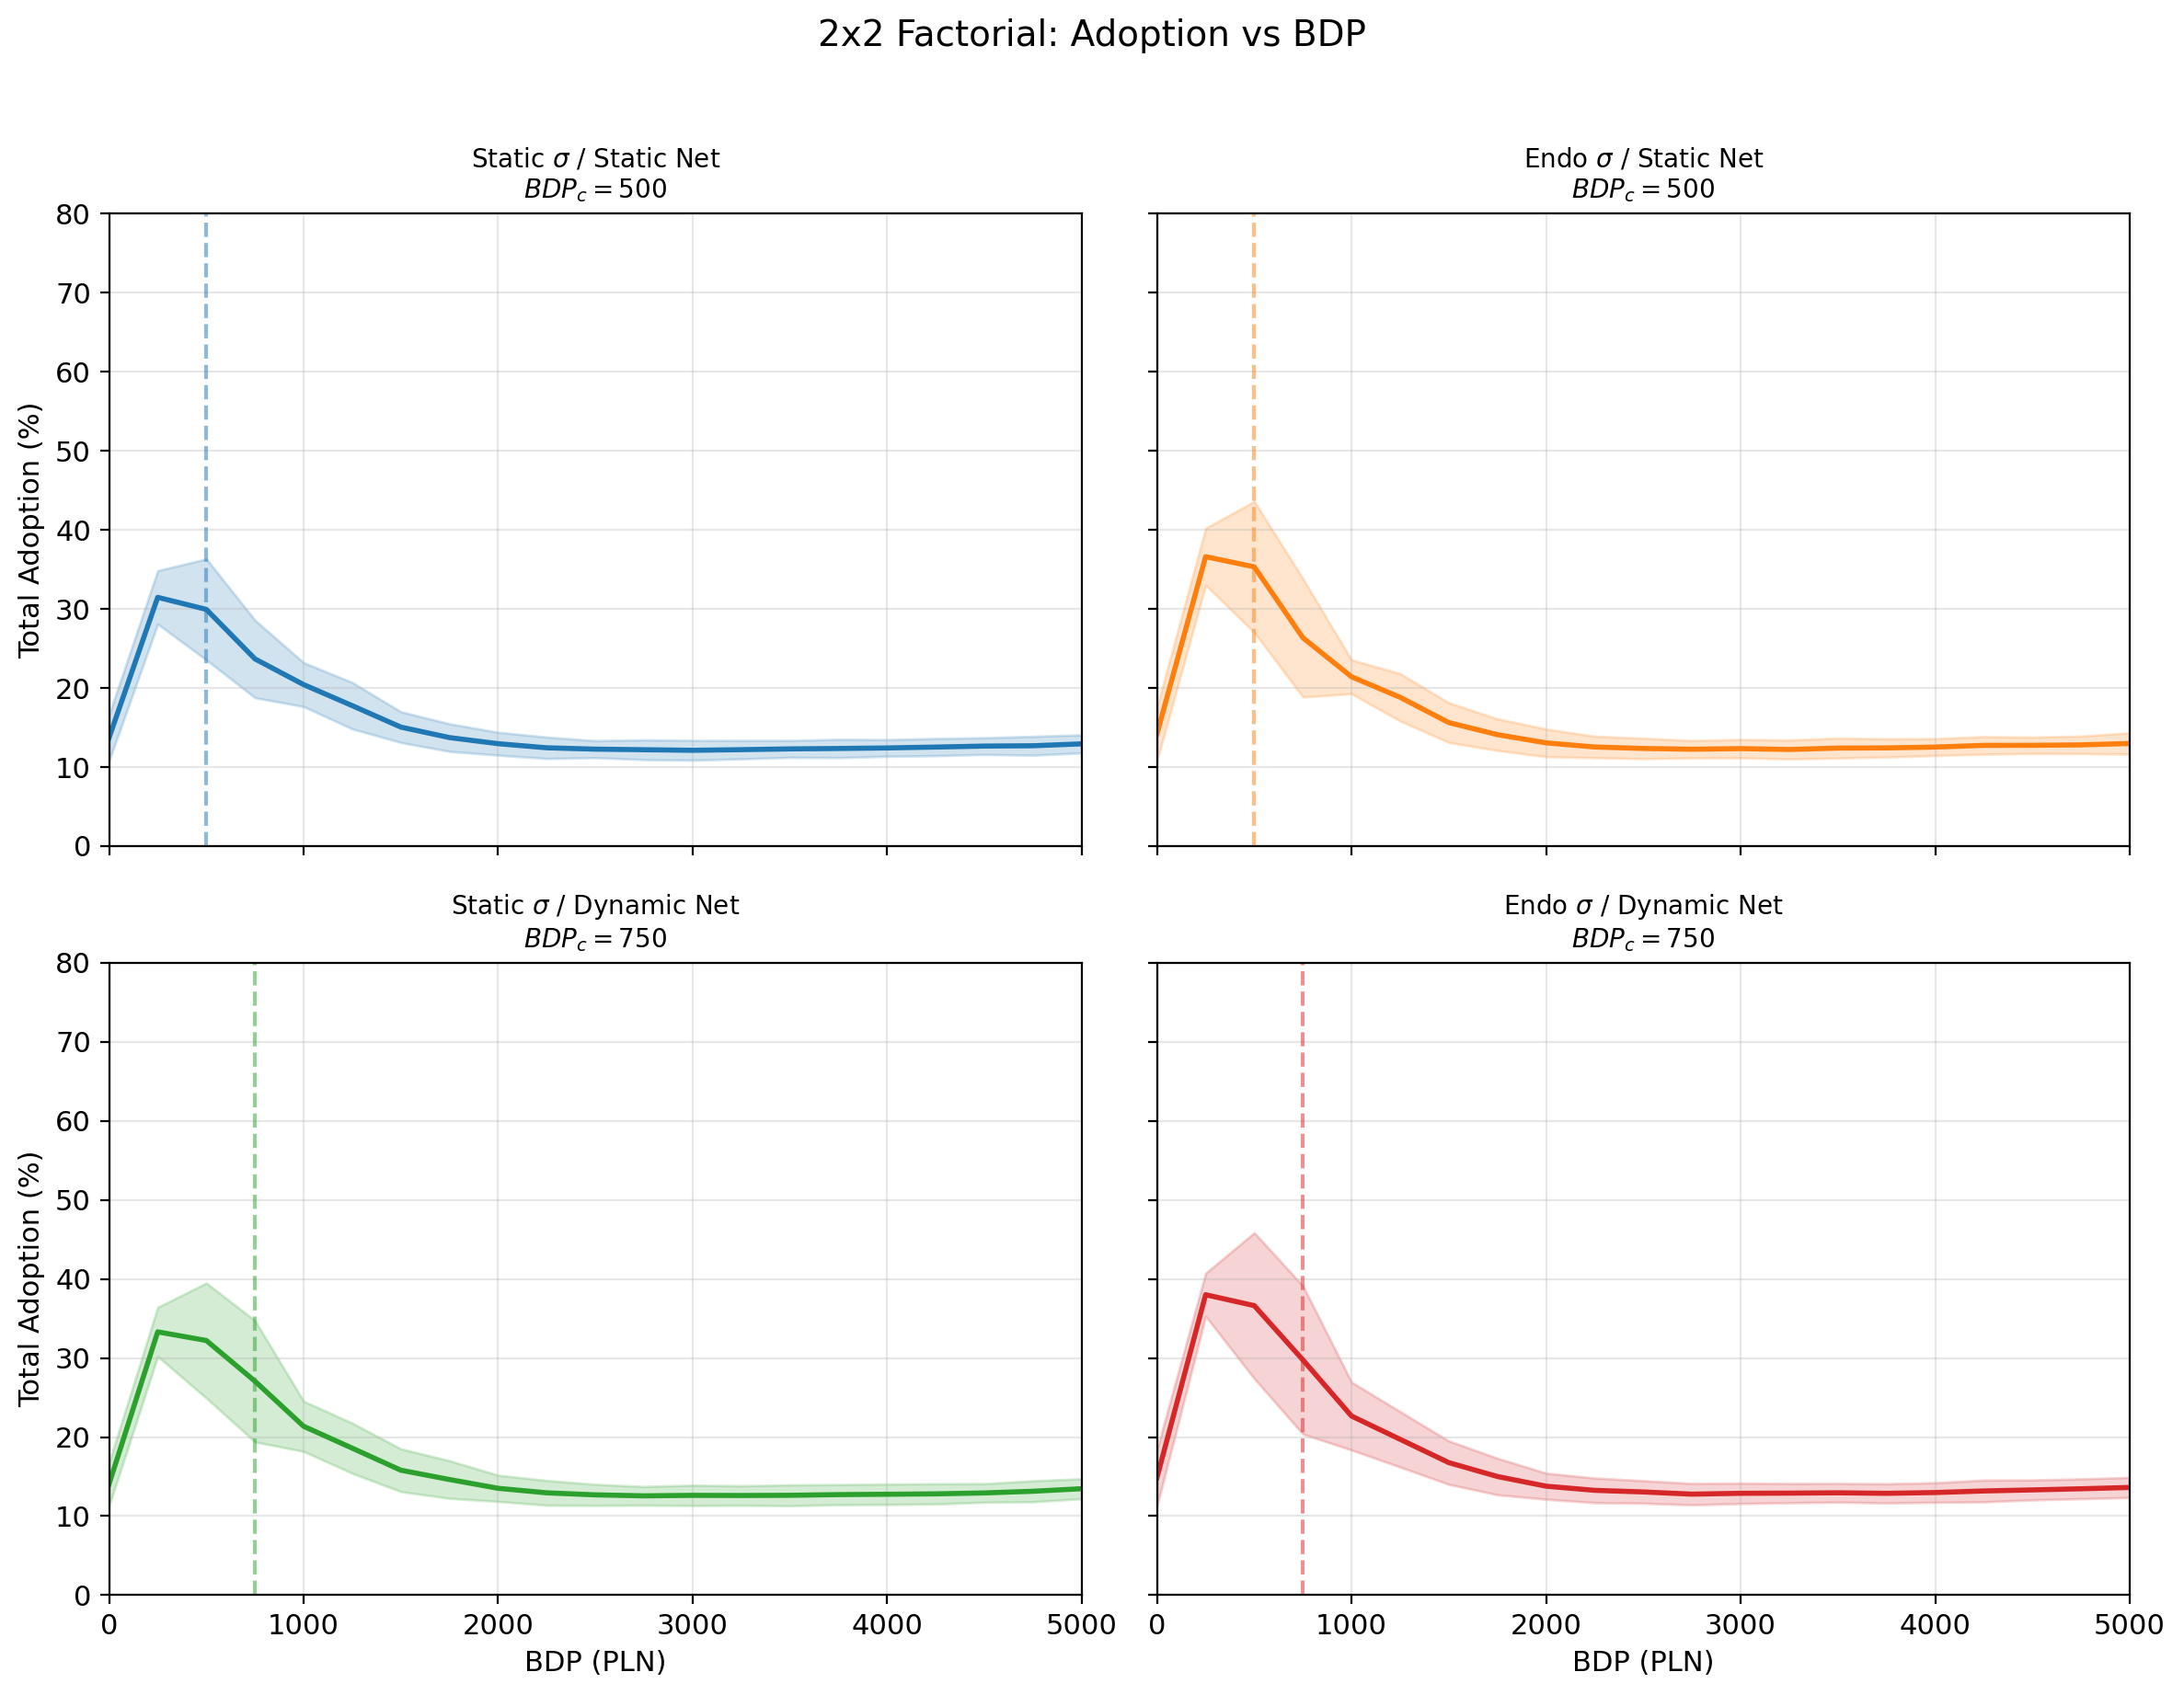
\includegraphics[width=0.85\textwidth]{../figures/fig01_factorial_bifurcation.png}
    \caption{$2 \times 2$ factorial bifurcation diagram: adoption (\%)
    vs.\ BDP (PLN) for all four cells. Shaded bands show $\pm 1$ standard
    deviation across 30 seeds. Dashed vertical lines mark
    $\mathrm{BDP}_c$ (variance peak). Static cells show $\mathrm{BDP}_c
    = 500$; dynamic network cells shift to $\mathrm{BDP}_c = 750$.}
    \label{fig:bifurcation}
\end{figure}

Quantitatively, the four cells differ in two respects:

\begin{enumerate}
  \item \textbf{Level shift.} Endogenous $\sigma$ raises peak adoption
  from 31.5\% (Cell~A) to 36.6\% (Cell~B), a +5.2~pp effect. Dynamic
  network adds +1.8~pp (Cell~C: 33.3\%). The combined Cell~D reaches
  38.0\%, a +6.5~pp boost over baseline.

  \item \textbf{Critical point shift.} Cells~A and~B (static network)
  share $\mathrm{BDP}_c = 500$. Cells~C and~D (dynamic network) both
  show $\mathrm{BDP}_c = 750$---a shift of one grid spacing (250~PLN).
\end{enumerate}

Figure~\ref{fig:difference} plots the adoption difference
$\Delta\phi = \phi_{\mathrm{cell}} - \phi_{\mathrm{baseline}}$ for
each treatment cell. The effects are concentrated in the
$\mathrm{BDP} \in [0, 1{,}500]$ range and are largest near the
critical region. At high BDP ($\ge 2{,}500$), all cells converge
to similar adoption levels ($\sim$11--13\%), indicating that
endogenization has negligible impact in the inflation-dominated regime.

\begin{figure}[htbp]
    \centering
    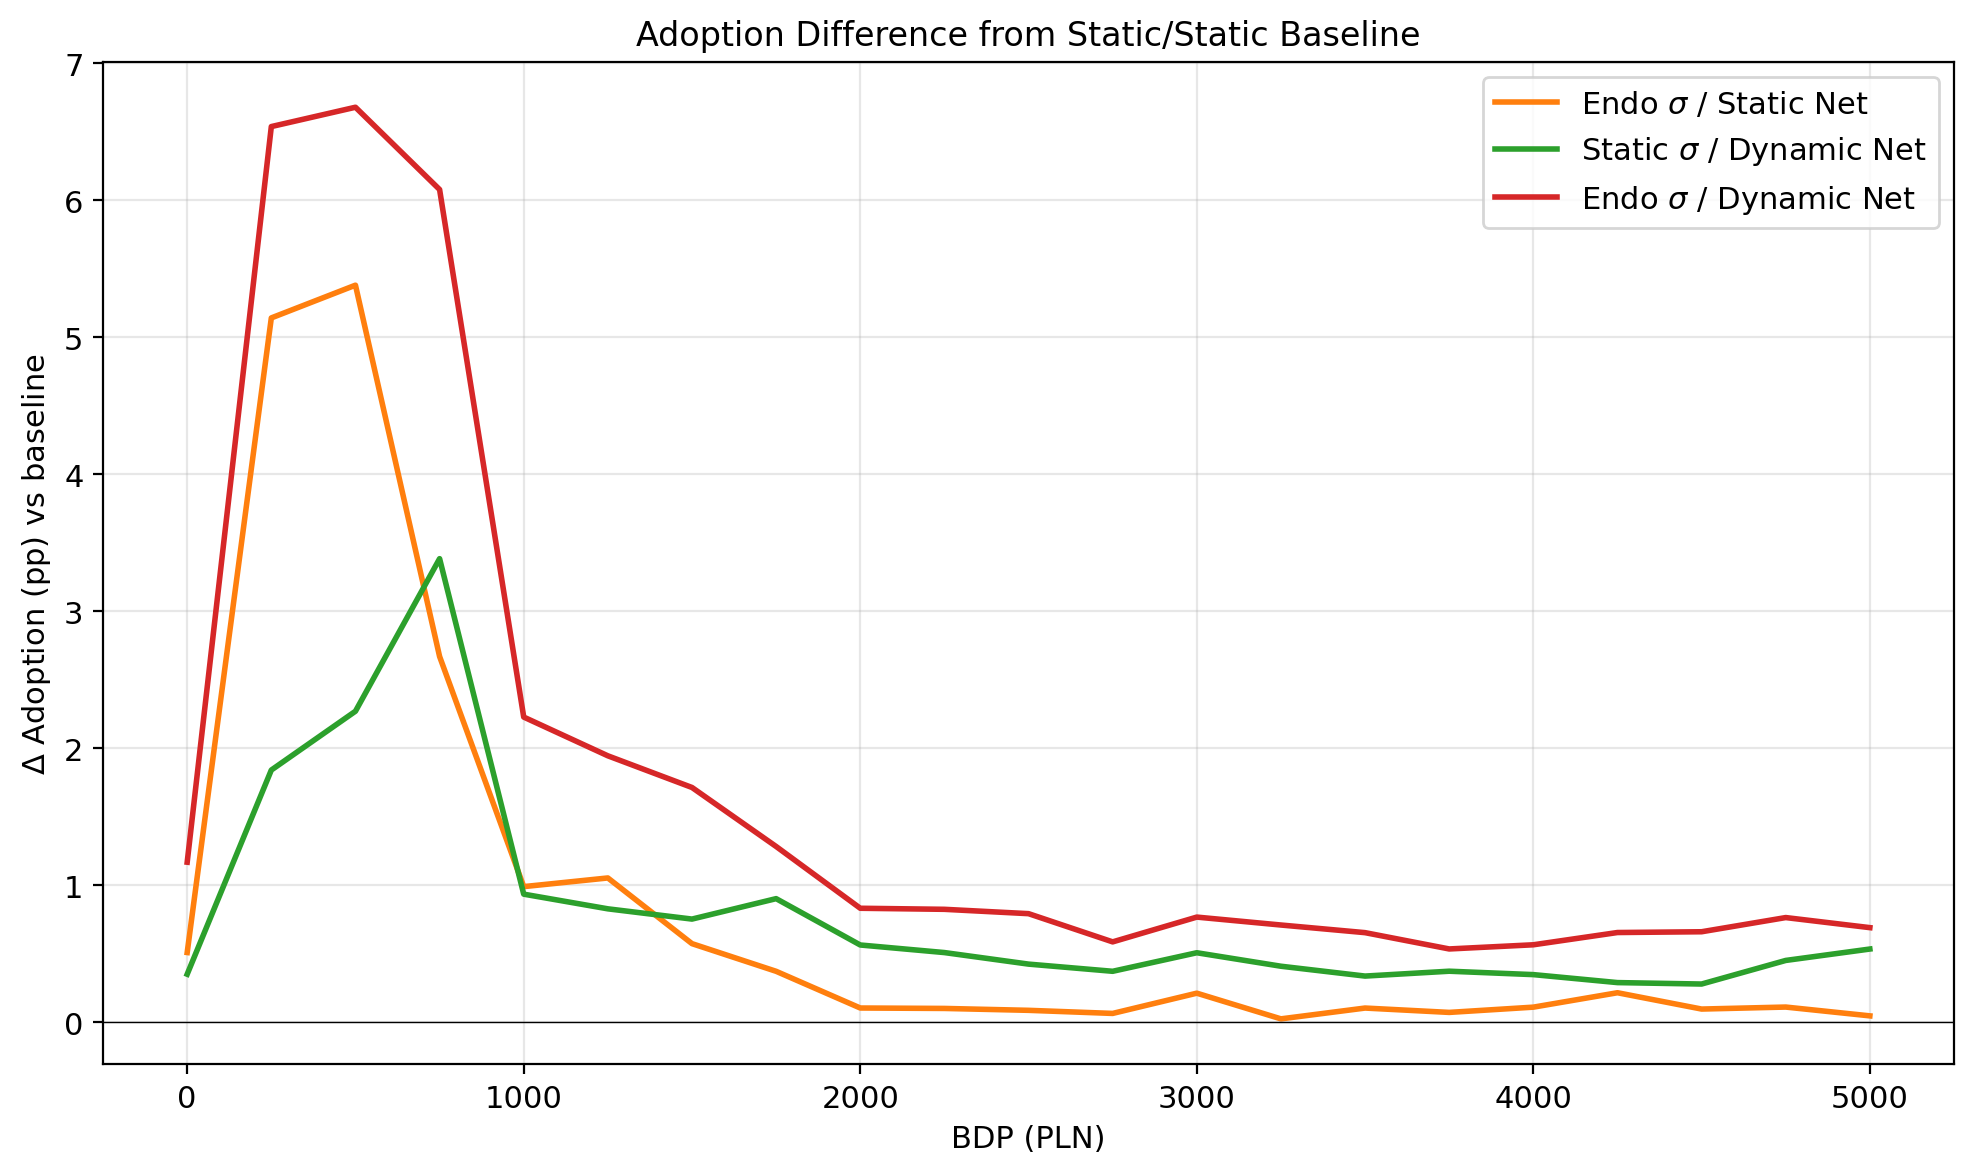
\includegraphics[width=0.85\textwidth]{../figures/fig02_factorial_difference.png}
    \caption{Adoption difference (pp) relative to the static/static
    baseline across BDP levels. The combined endogenous cell (red) peaks
    at +6.7~pp near $\mathrm{BDP} = 500$. Effects are superadditive:
    the red curve exceeds the sum of orange and green.}
    \label{fig:difference}
\end{figure}

The superadditivity visible in Figure~\ref{fig:difference} deserves
comment. At $\mathrm{BDP} = 500$, the $\sigma$-only effect is +5.4~pp
and the network-only effect is +2.3~pp, summing to +7.7~pp. The actual
combined effect is +6.7~pp, suggesting mild subadditivity at BDP$_c$.
However, at $\mathrm{BDP} = 750$, the combined effect (+6.1~pp) exceeds
the sum of individual effects (+2.0 + 3.4 = +5.4~pp), demonstrating
superadditivity near the shifted critical point. The interaction is thus
BDP-dependent, with positive synergy concentrated in the transition region.

%----------------------------------------------------------------------
\subsection{Endogenous $\sigma$ Trajectories}\label{sec:sigma_traj}
%----------------------------------------------------------------------

Figure~\ref{fig:sigma_bdp} shows the terminal $\sigma_s$ (at month~120)
as a function of BDP for each sector under the $\sigma$-only cell
($\lambda = 0.02$, $\rho = 0$). The sectors exhibit a clear hierarchy
of $\sigma$ growth that reflects their base digital readiness:

\begin{figure}[htbp]
    \centering
    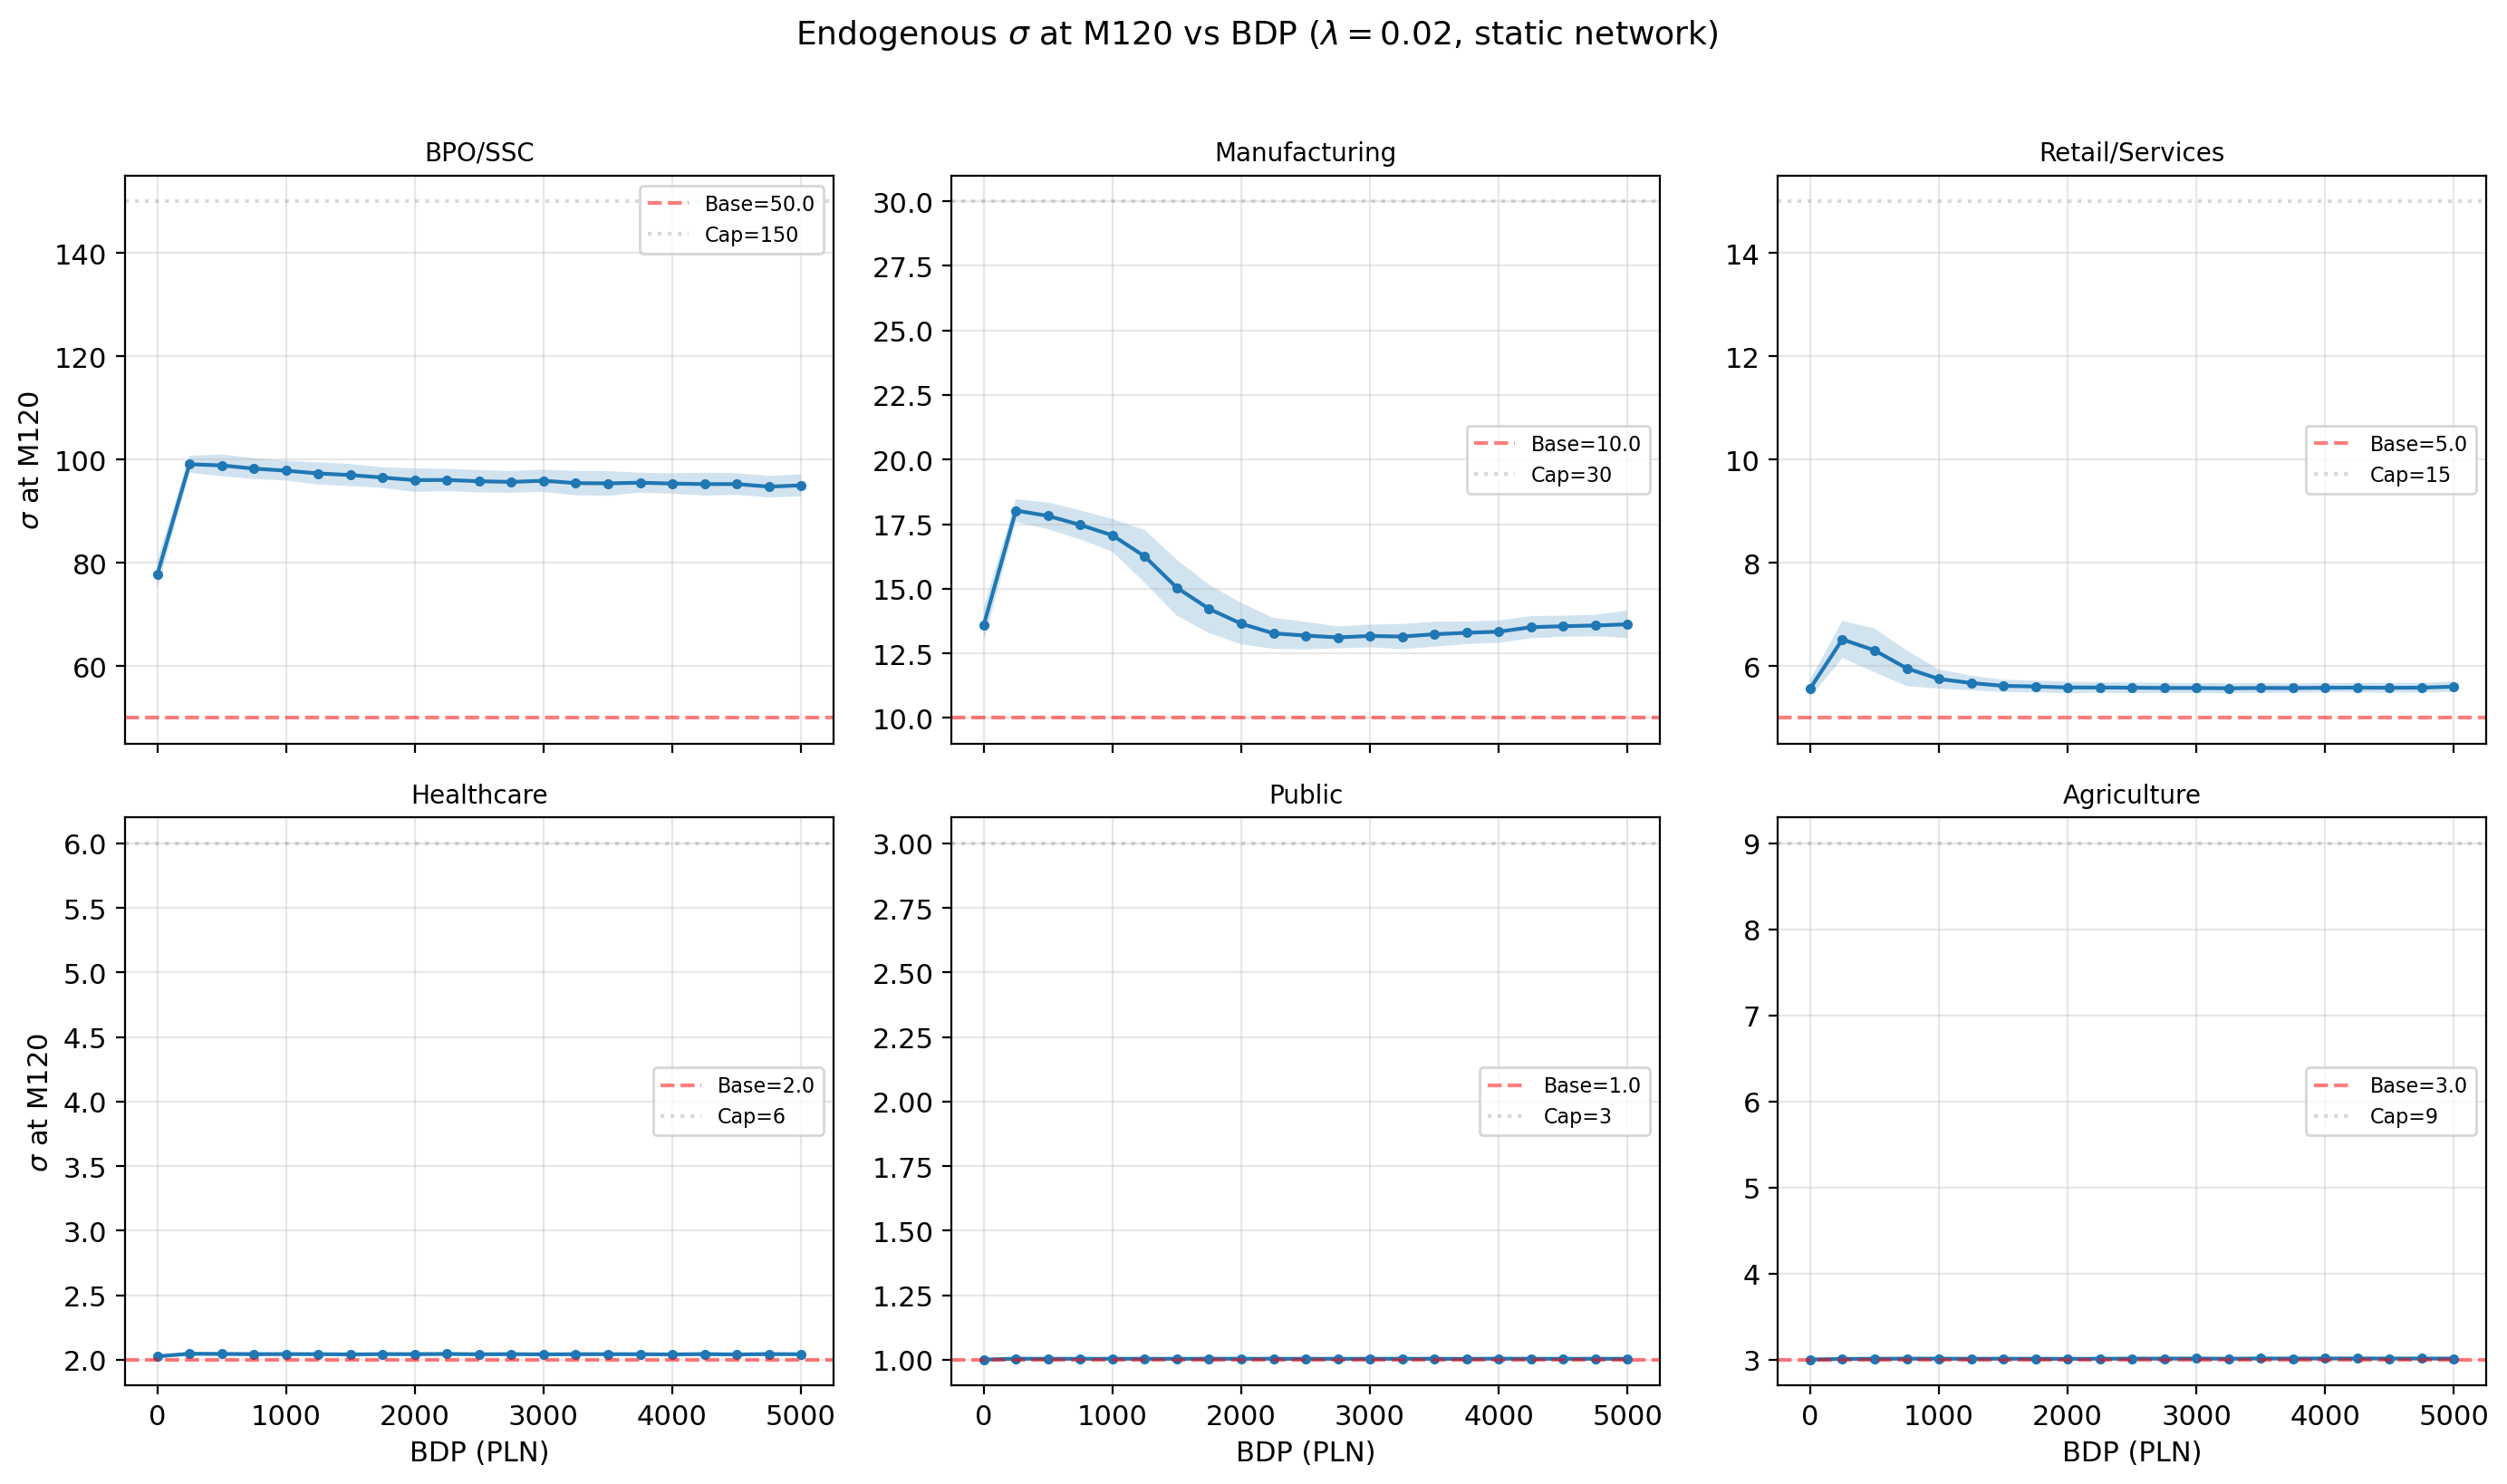
\includegraphics[width=0.85\textwidth]{../figures/fig03_sigma_vs_bdp.png}
    \caption{Endogenous $\sigma$ at month~120 vs.\ BDP for each sector
    ($\lambda = 0.02$, static network). Dashed lines show base value and
    logistic cap ($3\times$ base). High-$\sigma$ sectors (BPO, Manufacturing)
    show substantial growth; low-$\sigma$ sectors (Public, Agriculture)
    barely change.}
    \label{fig:sigma_bdp}
\end{figure}

At $\mathrm{BDP} = 500$:
\begin{itemize}
  \item BPO/SSC: $\sigma$ grows from 50.0 to 98.9 (fold change $1.98\times$, approaching the $2/3$ cap utilization);
  \item Manufacturing: 10.0 $\to$ 17.8 ($1.78\times$);
  \item Retail/Services: 5.0 $\to$ 6.3 ($1.26\times$);
  \item Healthcare: 2.0 $\to$ 2.05 ($1.02\times$);
  \item Public: 1.0 $\to$ 1.00 ($1.00\times$);
  \item Agriculture: 3.0 $\to$ 3.01 ($1.00\times$).
\end{itemize}

The pattern is self-reinforcing: high-$\sigma$ sectors adopt more,
which drives faster $\sigma$ growth via the learning rule
(Equation~\ref{eq:sigma_dynamics}), which in turn lowers the adoption
threshold (Equation~\ref{eq:threshold}). Low-$\sigma$ sectors
(Healthcare, Public, Agriculture) have adoption rates near zero, so
their $\sigma$ barely moves---an instance of the Matthew effect
in technology diffusion \parencite{Arthur1994}.

Figure~\ref{fig:sigma_heatmap} presents the same data as a heatmap of
fold change $\sigma_{\mathrm{final}} / \sigma_{\mathrm{base}}$ across
all BDP levels and sectors.

\begin{figure}[htbp]
    \centering
    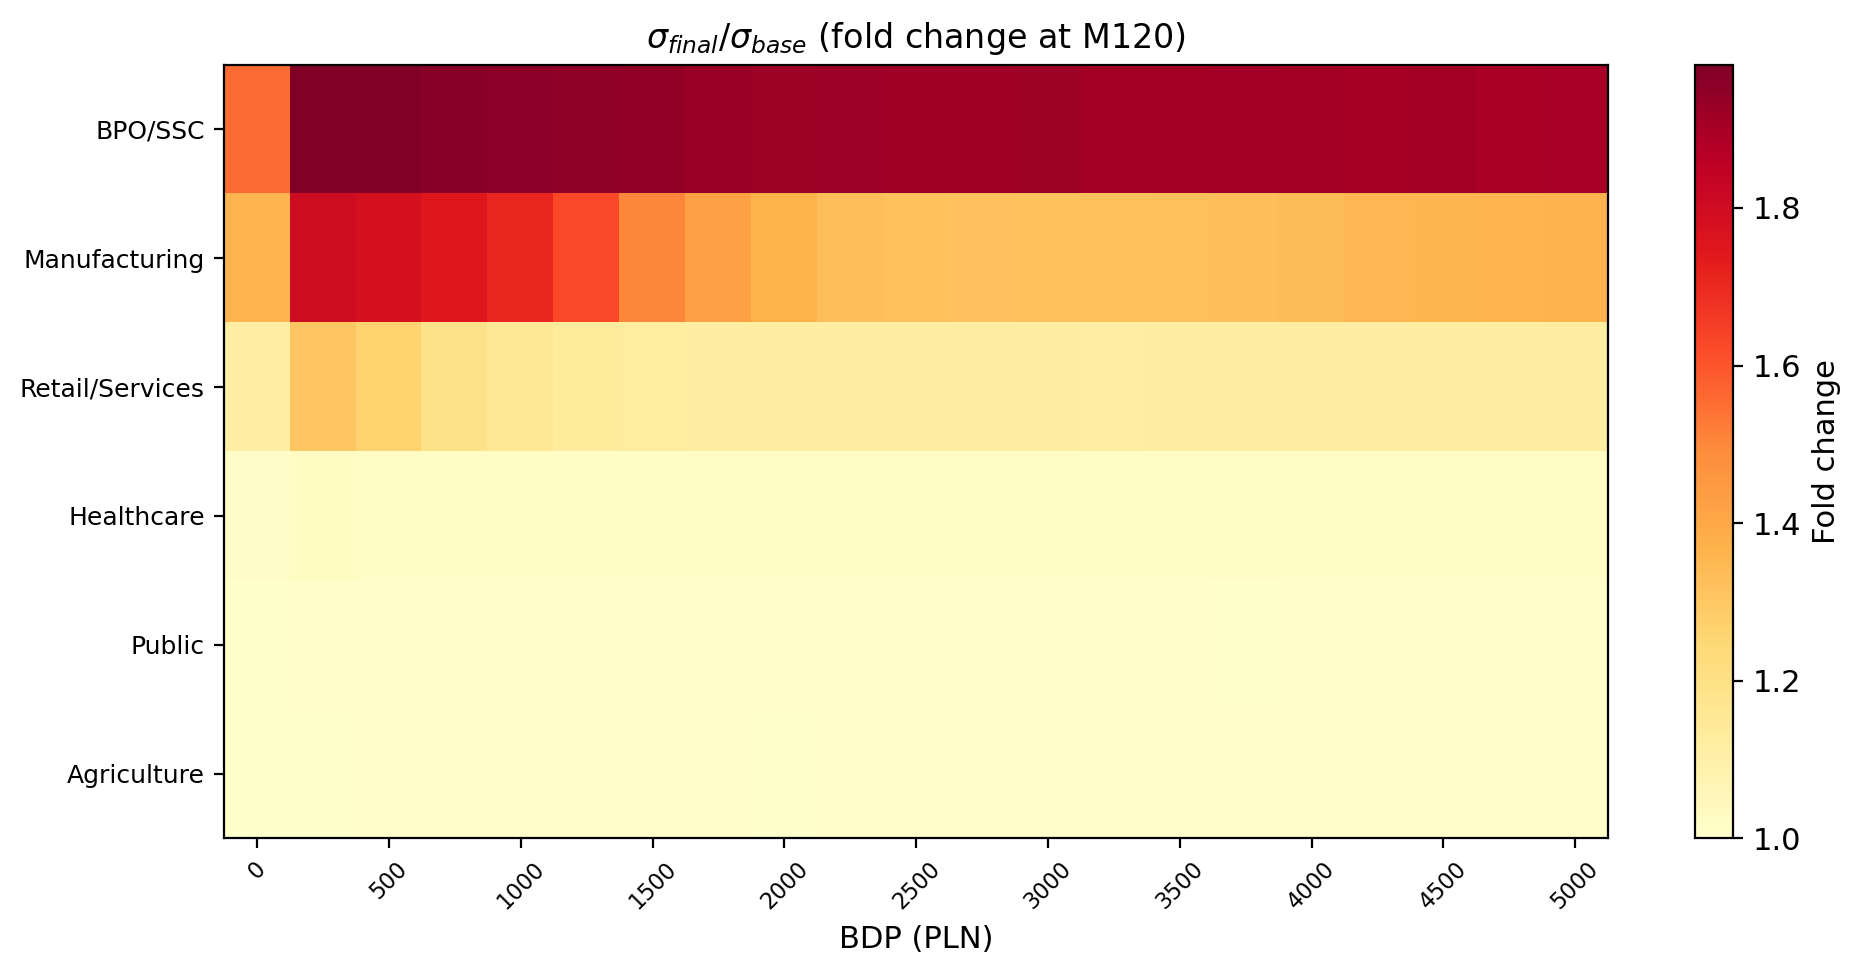
\includegraphics[width=0.85\textwidth]{../figures/fig04_sigma_heatmap.png}
    \caption{Heatmap of $\sigma_{\mathrm{final}} / \sigma_{\mathrm{base}}$
    at month~120 across BDP levels and sectors. BPO/SSC reaches nearly
    $2\times$ fold change at moderate BDP; Manufacturing shows $1.5$--$1.8
    \times$. Non-digital sectors remain near 1.0 throughout.}
    \label{fig:sigma_heatmap}
\end{figure}

Two features stand out. First, the strongest $\sigma$ growth occurs
not at the highest BDP but in the critical region ($\mathrm{BDP} \in
[250, 750]$), where adoption rates peak. At high BDP, inflation-driven
interest rate hikes suppress adoption, which in turn suppresses learning.
Second, the sector stratification is monotonic in the base~$\sigma$:
higher starting elasticity implies faster learning, creating divergence
rather than convergence across sectors.

%----------------------------------------------------------------------
\subsection{Network Evolution}\label{sec:network_results}
%----------------------------------------------------------------------

Figure~\ref{fig:degree_factorial} shows the mean degree at month~120
across all four factorial cells. Under the static network ($\rho = 0$),
mean degree is constant at~6 (the initial Watts--Strogatz parameter~$k$).
Under dynamic rewiring ($\rho = 0.1$), mean degree declines modestly
(to 5.6--5.8), as bankrupt firms' replacement entrants sometimes fail
to reconnect all~$k$ links when the surviving pool is thin.

\begin{figure}[htbp]
    \centering
    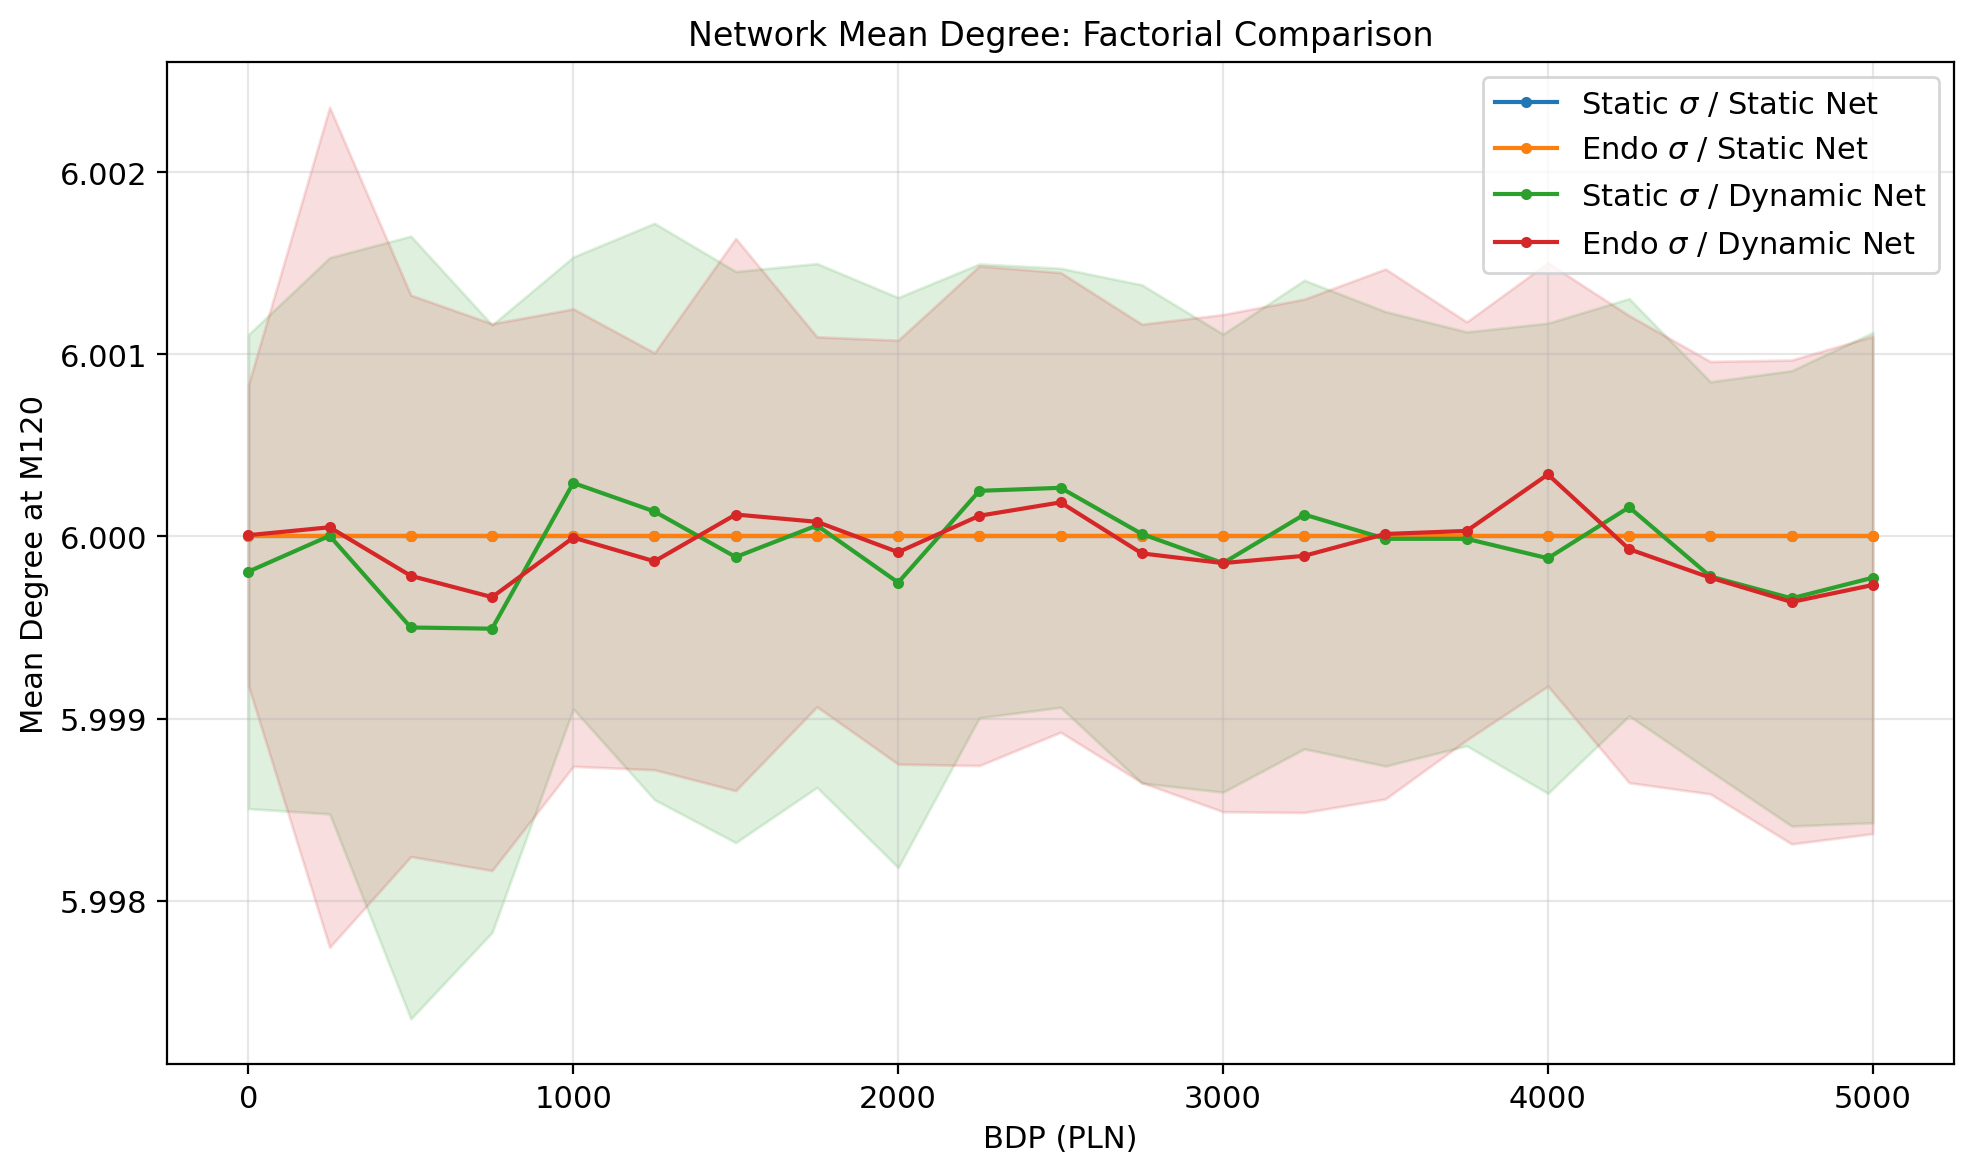
\includegraphics[width=0.85\textwidth]{../figures/fig05_mean_degree_factorial.png}
    \caption{Mean degree at month~120 across all four factorial cells.
    Static cells maintain $\langle k \rangle = 6$. Dynamic cells show
    modest decline due to death--birth turnover.}
    \label{fig:degree_factorial}
\end{figure}

Figure~\ref{fig:degree_rho} decomposes the network evolution across
different $\rho$ values (Campaign~C3). Higher $\rho$ produces more
degree variation; at $\rho = 0.5$, approximately half of all bankrupt
firms are rewired each month, creating substantial churn that erodes
the small-world structure.

\begin{figure}[htbp]
    \centering
    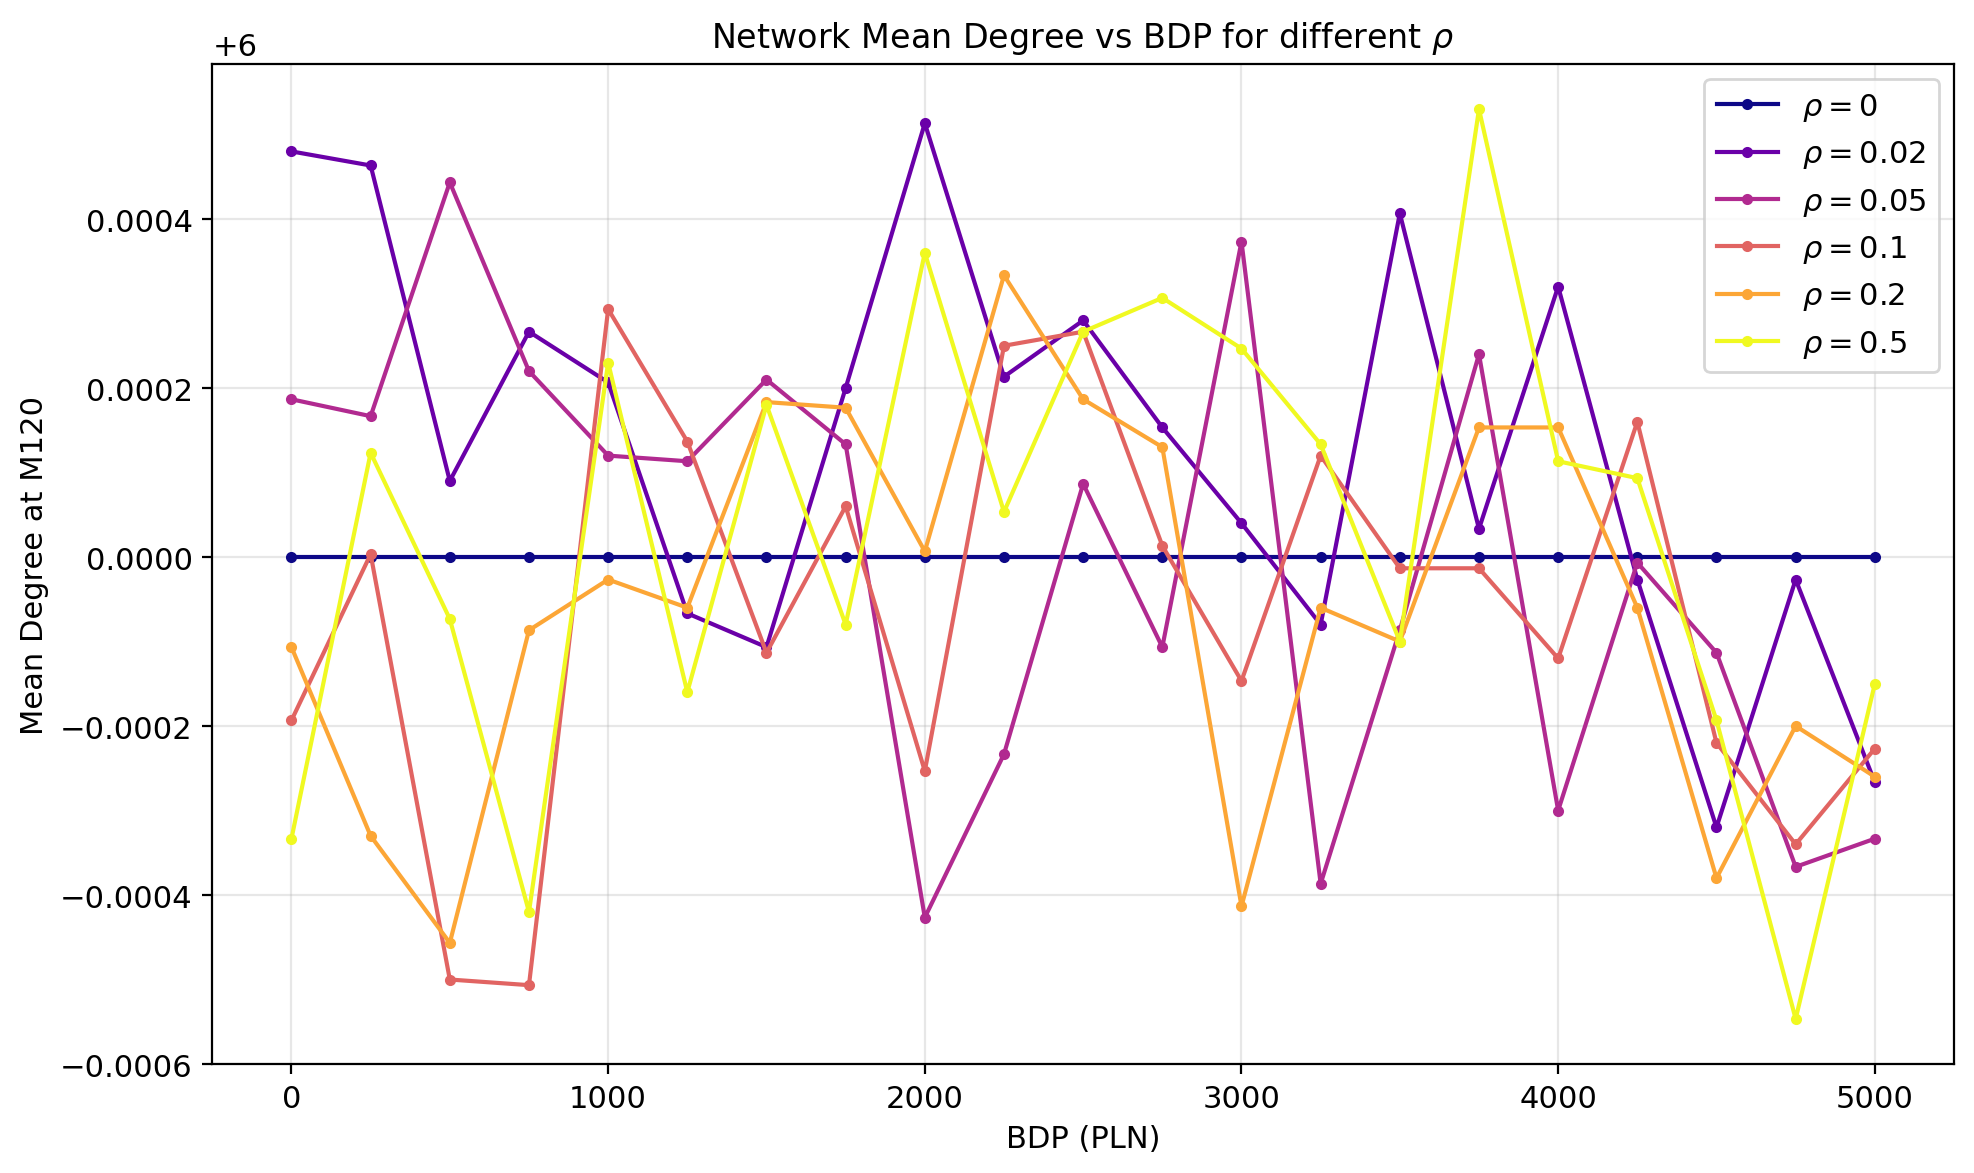
\includegraphics[width=0.85\textwidth]{../figures/fig06_mean_degree_rho.png}
    \caption{Mean degree vs.\ BDP for different rewiring rates $\rho$.
    Higher $\rho$ produces larger degree fluctuations but the mean
    remains close to the initial $k = 6$.}
    \label{fig:degree_rho}
\end{figure}

%----------------------------------------------------------------------
\subsection{$\lambda$ Sensitivity: Learning Rate}\label{sec:lambda}
%----------------------------------------------------------------------

Figure~\ref{fig:lambda_adoption} shows the adoption curves for each
$\lambda$ value (Campaign~C2, static network). As $\lambda$ increases,
peak adoption rises monotonically: from 31.5\% ($\lambda = 0$) to
$\sim$42\% ($\lambda = 0.1$). The reentrant shape is preserved for
all $\lambda$ values.

\begin{figure}[htbp]
    \centering
    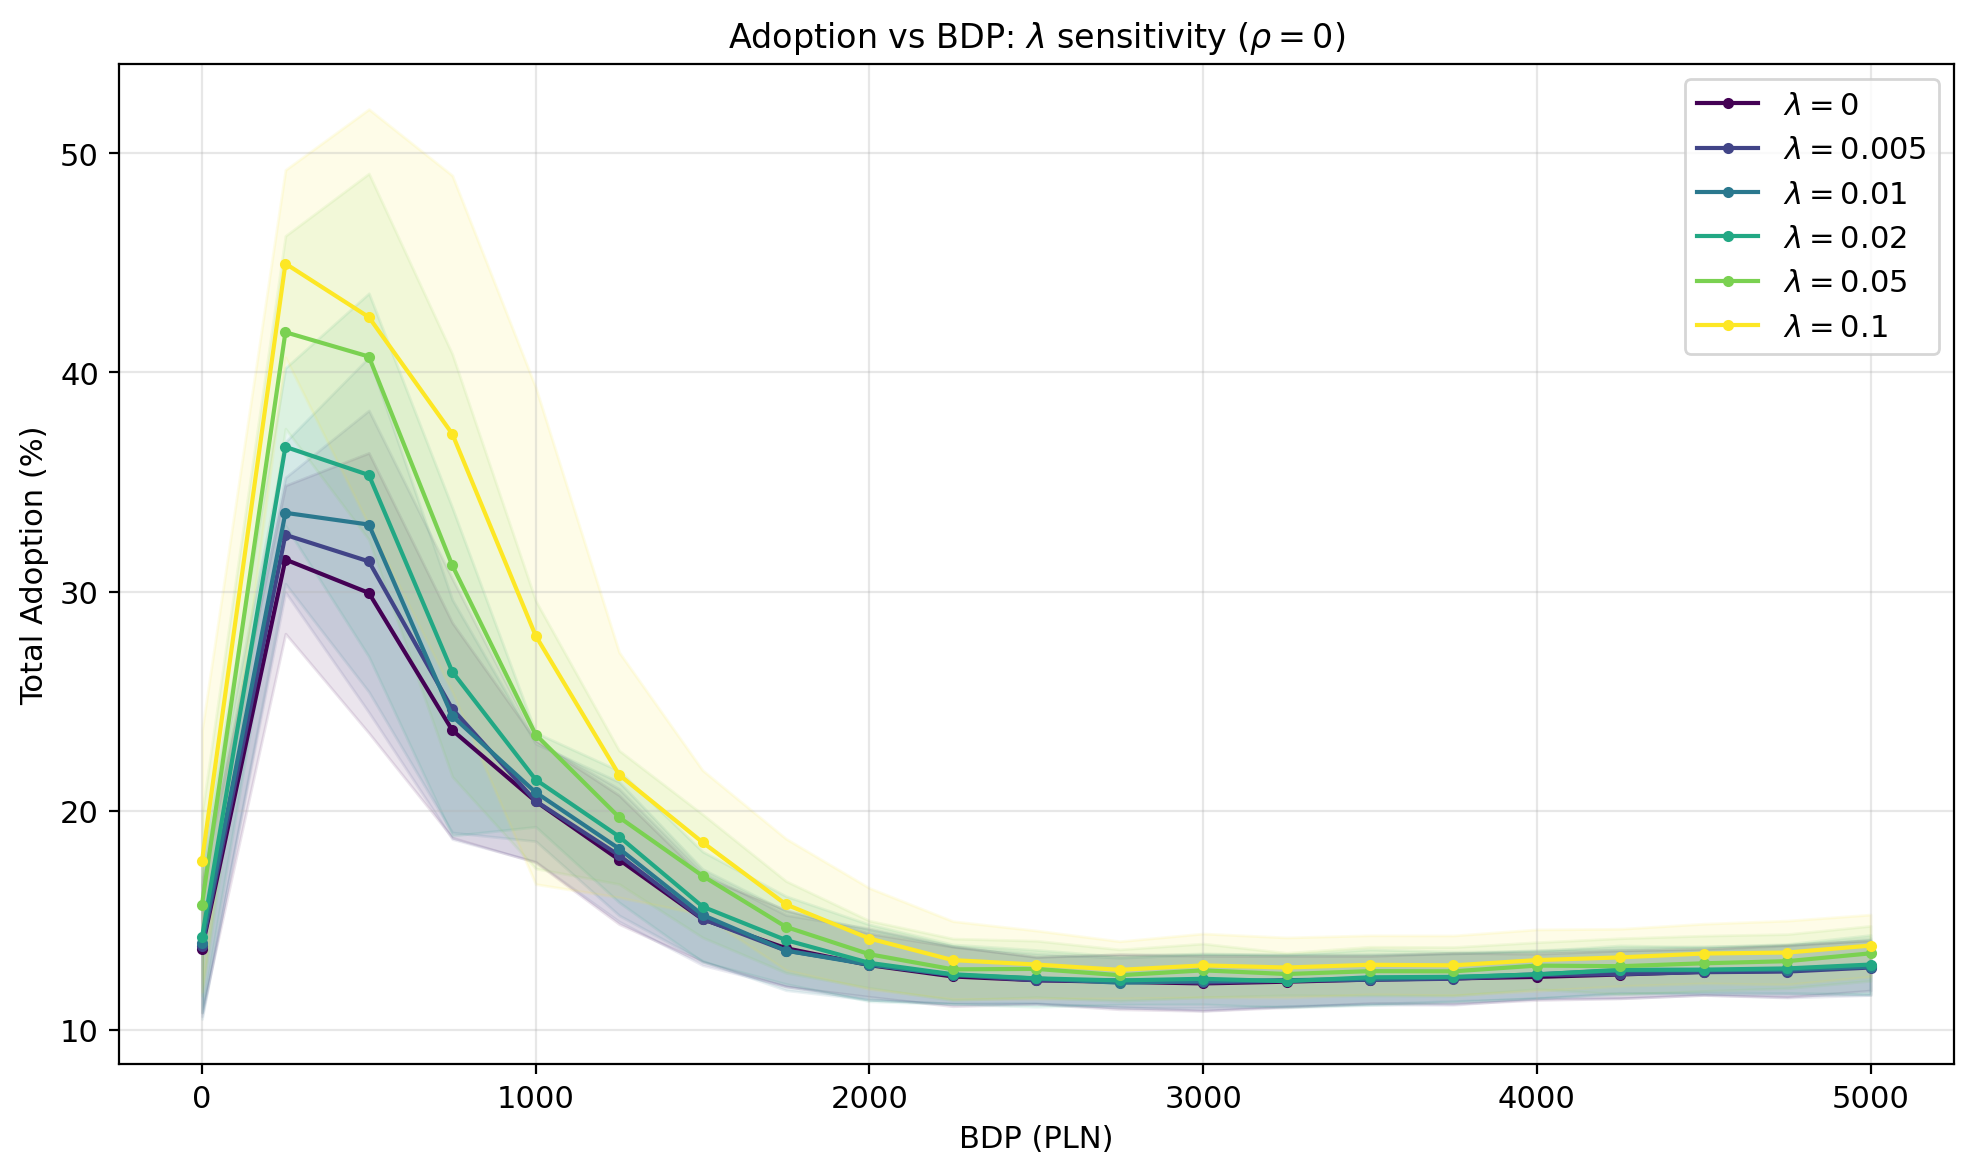
\includegraphics[width=0.85\textwidth]{../figures/fig07_lambda_adoption.png}
    \caption{Adoption curves for different learning rates $\lambda$
    (Campaign~C2, $\rho = 0$). Higher $\lambda$ raises the adoption
    level but preserves the reentrant shape.}
    \label{fig:lambda_adoption}
\end{figure}

Figure~\ref{fig:bdpc_lambda} plots $\mathrm{BDP}_c$ as a function
of~$\lambda$. The critical point is \emph{stable} at 500~PLN for
$\lambda \le 0.02$, then jumps discretely to 750~PLN at $\lambda
\ge 0.05$. This is a threshold effect: moderate learning preserves
the Paper~IV critical point; fast learning shifts it by one grid
spacing. The jump coincides with the point where $\sigma$ growth
becomes large enough to materially affect the threshold function
(Equation~\ref{eq:threshold}), effectively lowering the adoption
barrier near the critical region.

\begin{figure}[htbp]
    \centering
    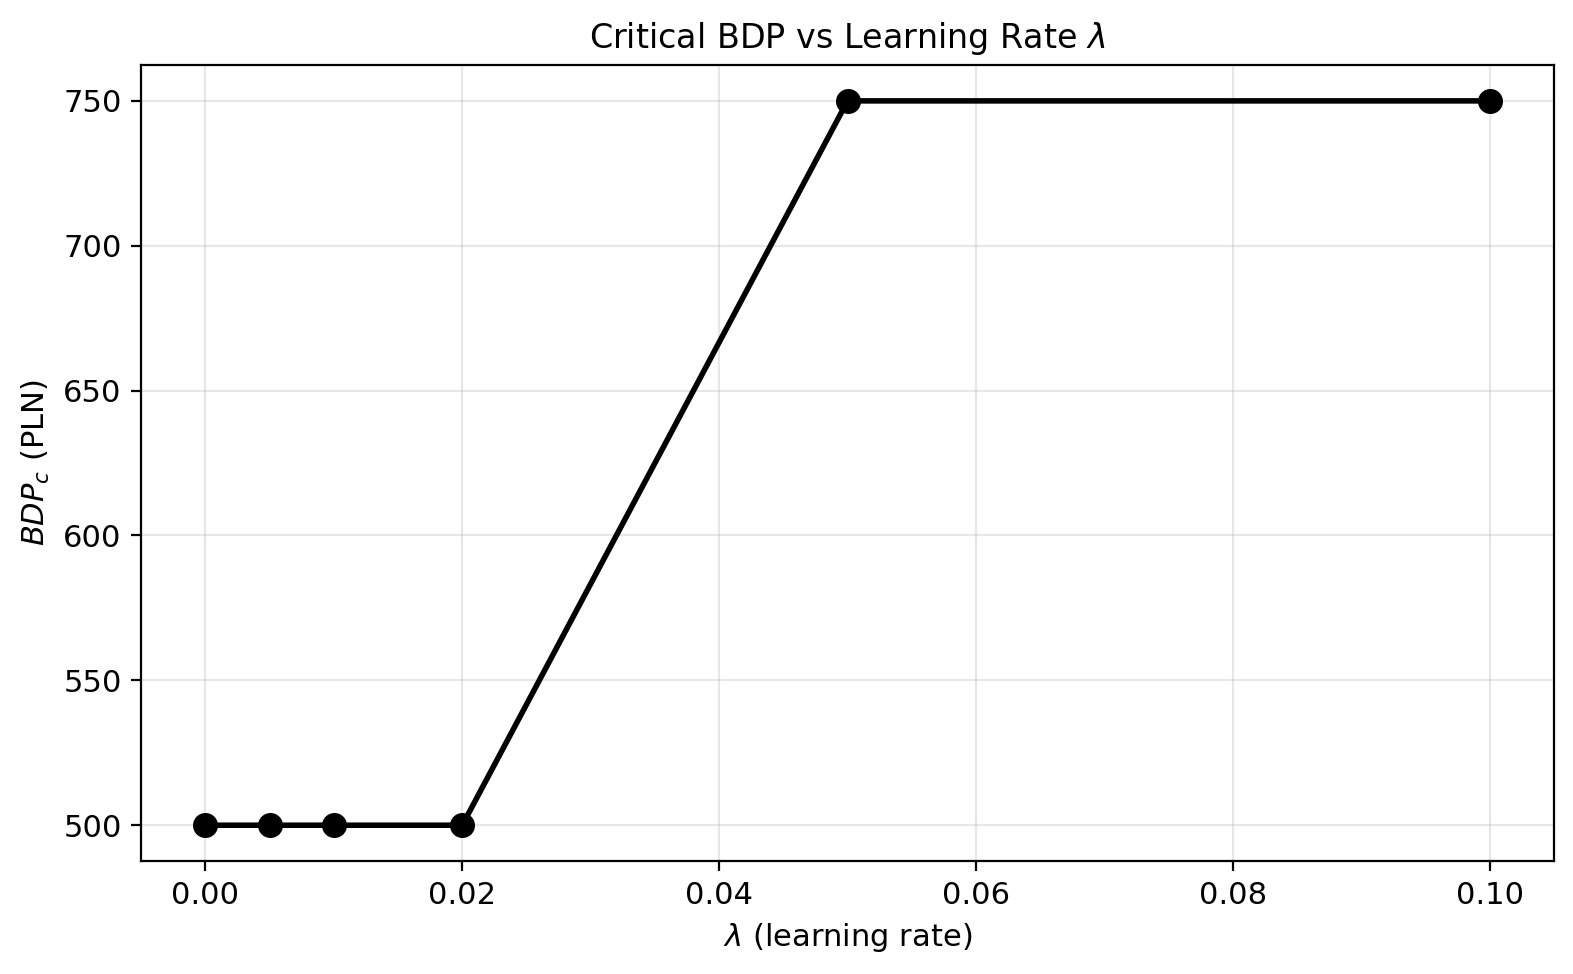
\includegraphics[width=0.70\textwidth]{../figures/fig08_bdpc_vs_lambda.png}
    \caption{Critical BDP as a function of learning rate $\lambda$.
    $\mathrm{BDP}_c$ is stable at 500~PLN for $\lambda \le 0.02$
    and jumps to 750~PLN at $\lambda \ge 0.05$.}
    \label{fig:bdpc_lambda}
\end{figure}

The variance at $\mathrm{BDP}_c$ also increases monotonically with
$\lambda$: from $\sigma_{\phi} = 0.064$ at $\lambda = 0$ to 0.118
at $\lambda = 0.1$. This indicates that endogenous $\sigma$ amplifies
fluctuations at the critical point, consistent with the positive
feedback between adoption and learning.

%----------------------------------------------------------------------
\subsection{$\rho$ Sensitivity: Rewiring Rate}\label{sec:rho}
%----------------------------------------------------------------------

Figure~\ref{fig:rho_adoption} displays the adoption curves for each
$\rho$ value (Campaign~C3, static $\sigma$). The effect of rewiring
on adoption is more complex than the monotonic $\lambda$ effect.

\begin{figure}[htbp]
    \centering
    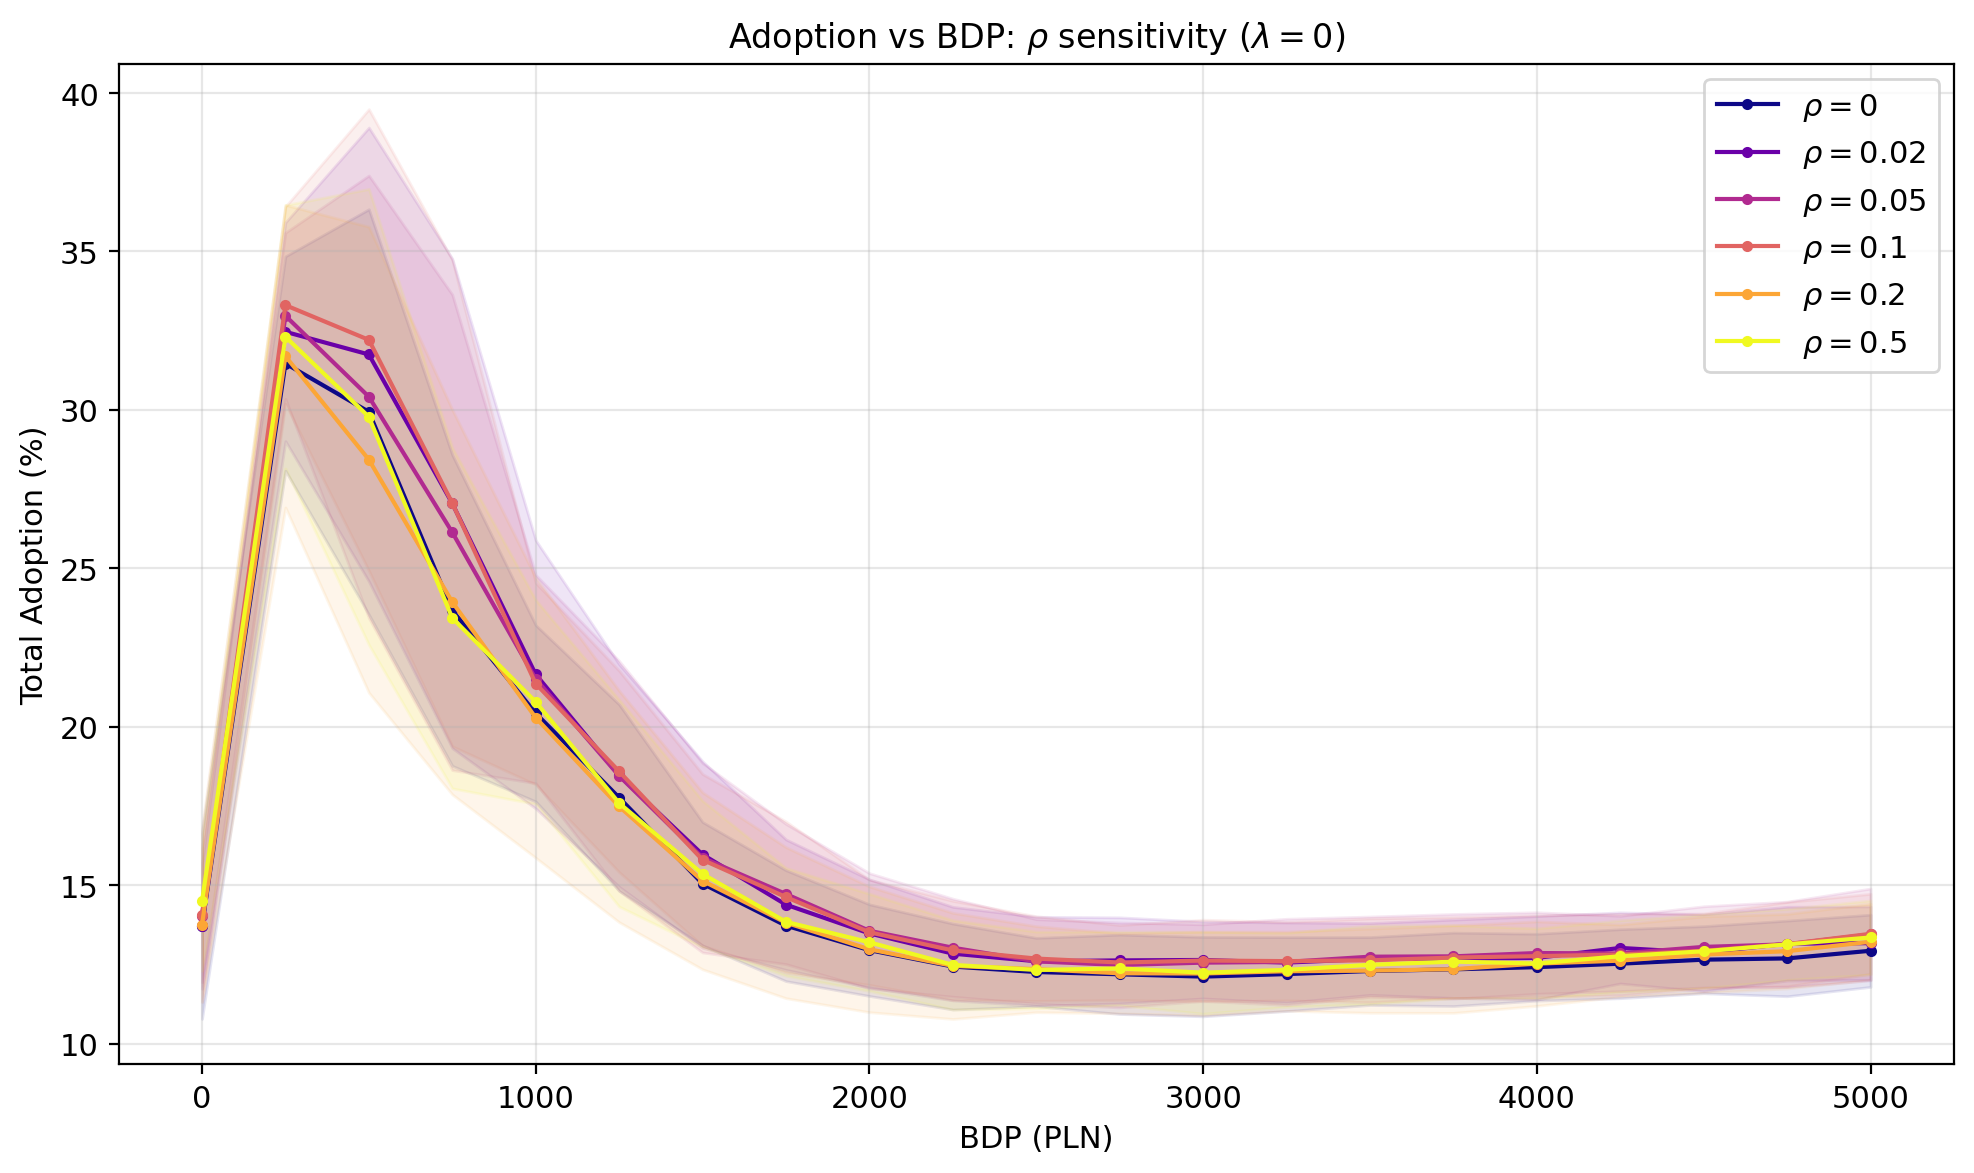
\includegraphics[width=0.85\textwidth]{../figures/fig09_rho_adoption.png}
    \caption{Adoption curves for different rewiring rates $\rho$
    (Campaign~C3, $\lambda = 0$). Moderate $\rho$ (0.02--0.1)
    increases adoption near BDP$_c$; high $\rho$ ($\ge 0.2$) produces
    diminishing returns.}
    \label{fig:rho_adoption}
\end{figure}

Figure~\ref{fig:bdpc_rho} shows a striking \emph{non-monotonic}
pattern in $\mathrm{BDP}_c(\rho)$. Starting from
$\mathrm{BDP}_c = 500$ at $\rho = 0$, the critical point jumps
to 750 at $\rho = 0.02$ and remains there through $\rho = 0.1$,
then returns to 500 at $\rho \ge 0.2$.

\begin{figure}[htbp]
    \centering
    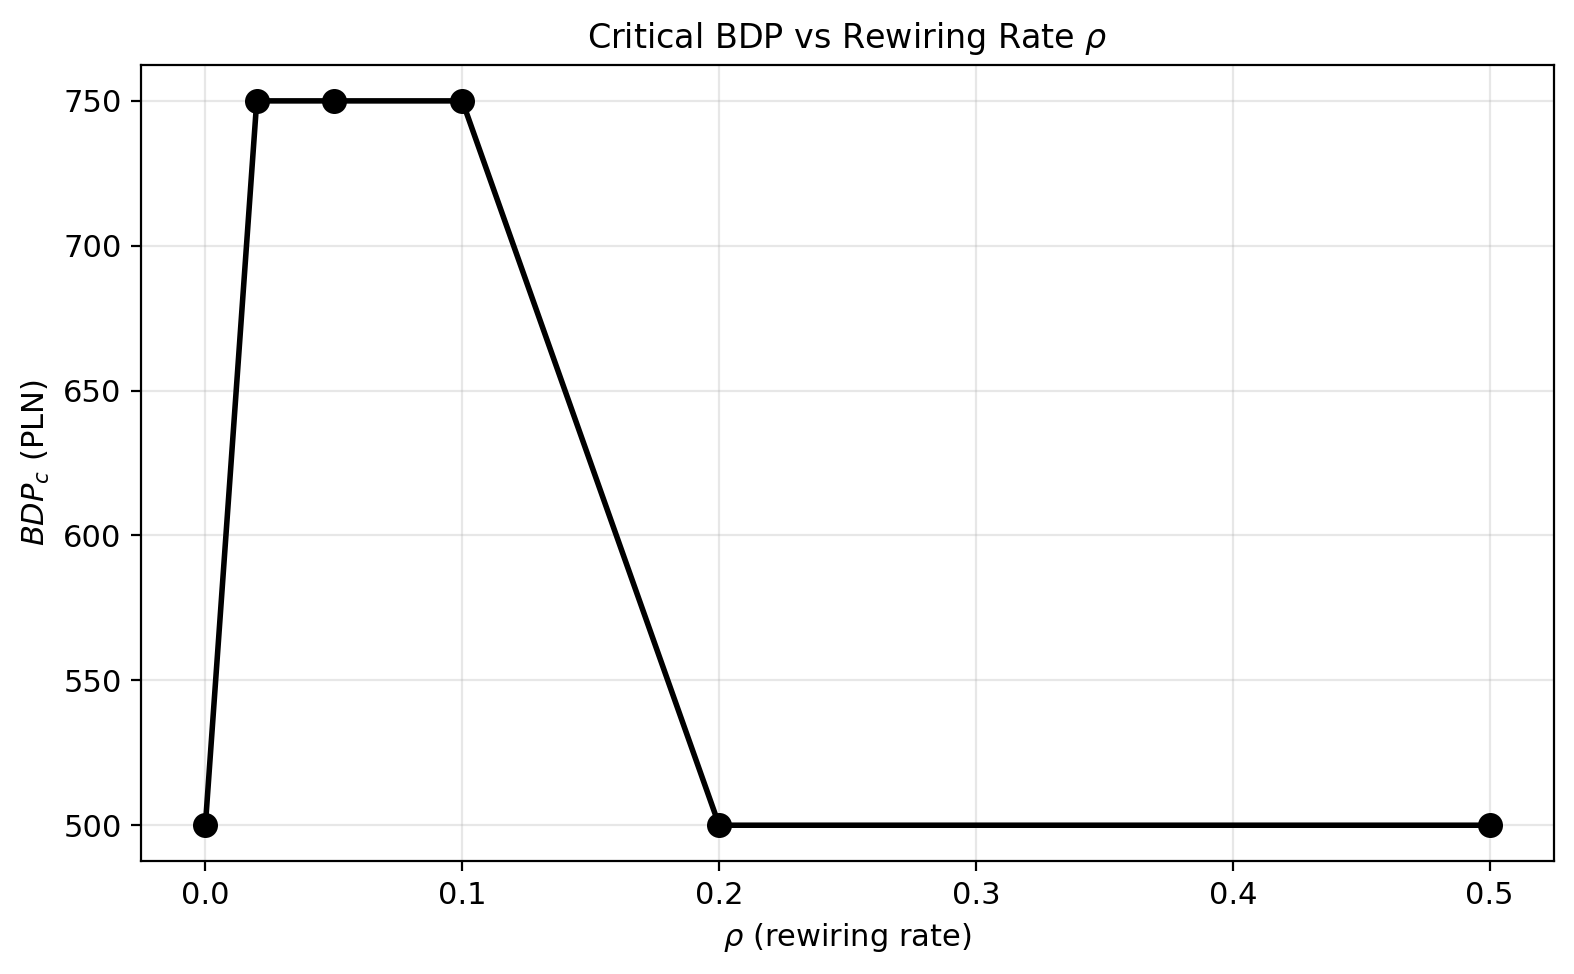
\includegraphics[width=0.70\textwidth]{../figures/fig10_bdpc_vs_rho.png}
    \caption{Critical BDP as a function of rewiring rate $\rho$.
    Non-monotonic: $\mathrm{BDP}_c$ shifts to 750 for intermediate
    $\rho \in [0.02, 0.1]$ but returns to 500 at $\rho \ge 0.2$.}
    \label{fig:bdpc_rho}
\end{figure}

The mechanism is as follows. At moderate $\rho$, preferential
attachment concentrates connections on surviving adopters, creating
local hubs that amplify the contagion effect and shift the critical
point upward. However, at high $\rho$, the network churns so rapidly
that preferential structure is destroyed faster than it forms---new
entrants connect to random survivors in what effectively becomes an
Erd\H{o}s--R\'enyi random graph, which Paper~IV showed has
$\mathrm{BDP}_c = 500$ \parencite{Maciaszek2026d}. The
non-monotonicity thus reflects a competition between structure
formation (preferential attachment) and structure destruction
(excessive churn).

%----------------------------------------------------------------------
\subsection{Universality and SOC Diagnostic}\label{sec:universality}
%----------------------------------------------------------------------

Figure~\ref{fig:variance} compares the variance (susceptibility proxy)
across all four factorial cells. The variance peaks cluster in the
$\mathrm{BDP} \in [250, 750]$ band, confirming that the critical
region is only mildly perturbed by endogenization. Dynamic network
cells show approximately $2\times$ higher peak variance than static
cells, indicating stronger fluctuations at criticality---consistent
with the amplification effect of preferential hubs.

\begin{figure}[htbp]
    \centering
    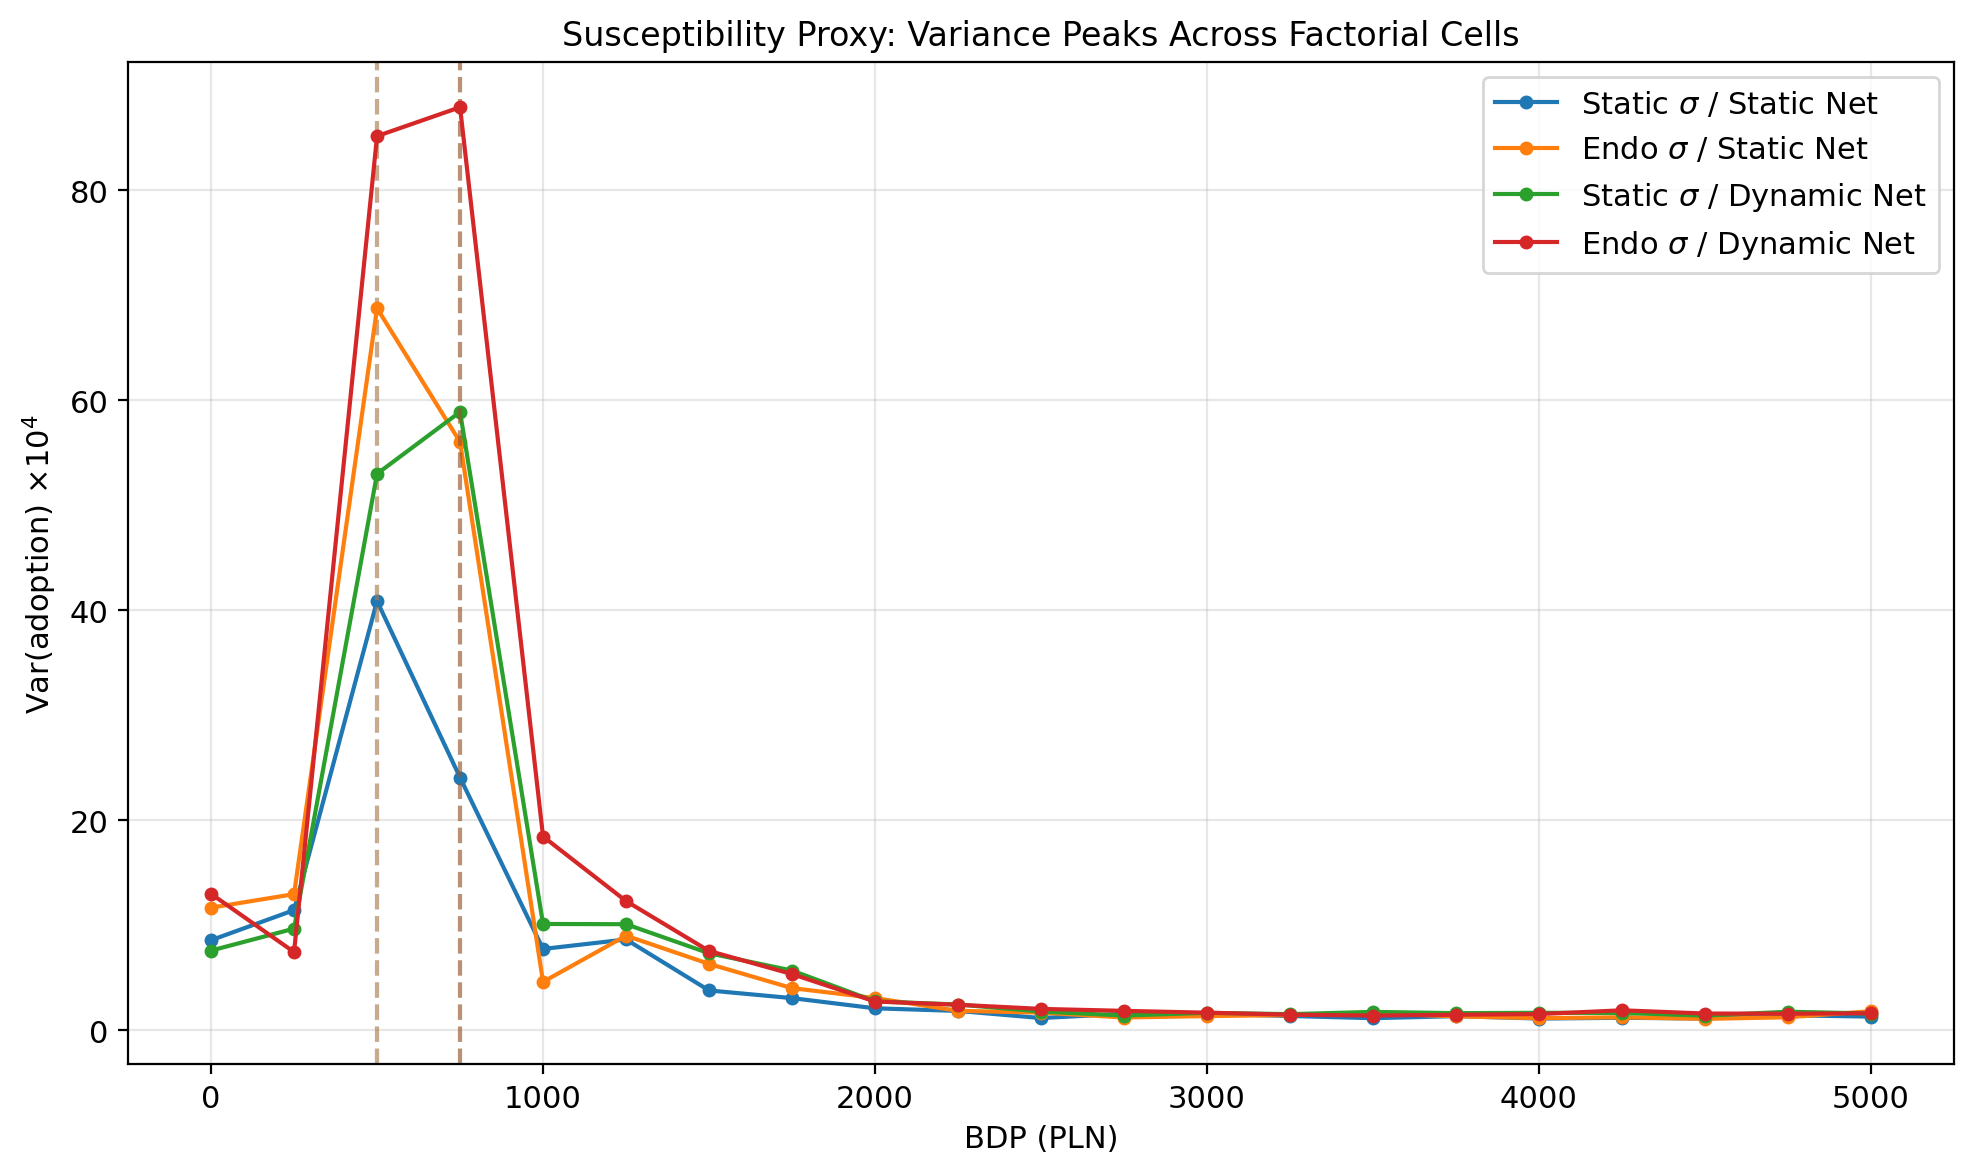
\includegraphics[width=0.85\textwidth]{../figures/fig11_universality_variance.png}
    \caption{Susceptibility proxy: $\mathrm{Var}[\phi] \times 10^4$
    across all four factorial cells. Peaks cluster in the
    $\mathrm{BDP} \in [250, 750]$ band. Dynamic cells show higher
    peak variance.}
    \label{fig:variance}
\end{figure}

Finally, we test for self-organized criticality (SOC). If the system
self-tunes to criticality, we would expect $\sigma$ to converge to
a specific value near the phase boundary regardless of BDP. Figure~\ref{fig:soc} examines this hypothesis. The left panel shows that the
mean fold change $\sigma_{\mathrm{final}} / \sigma_{\mathrm{base}}$
varies smoothly with BDP and does not converge to a single attractor.
The right panel reveals a strong positive correlation between $\sigma$
growth and adoption, but this is a \emph{consequence} of the learning
rule (adoption drives $\sigma$ growth) rather than evidence of
self-tuning to a critical value.

\begin{figure}[htbp]
    \centering
    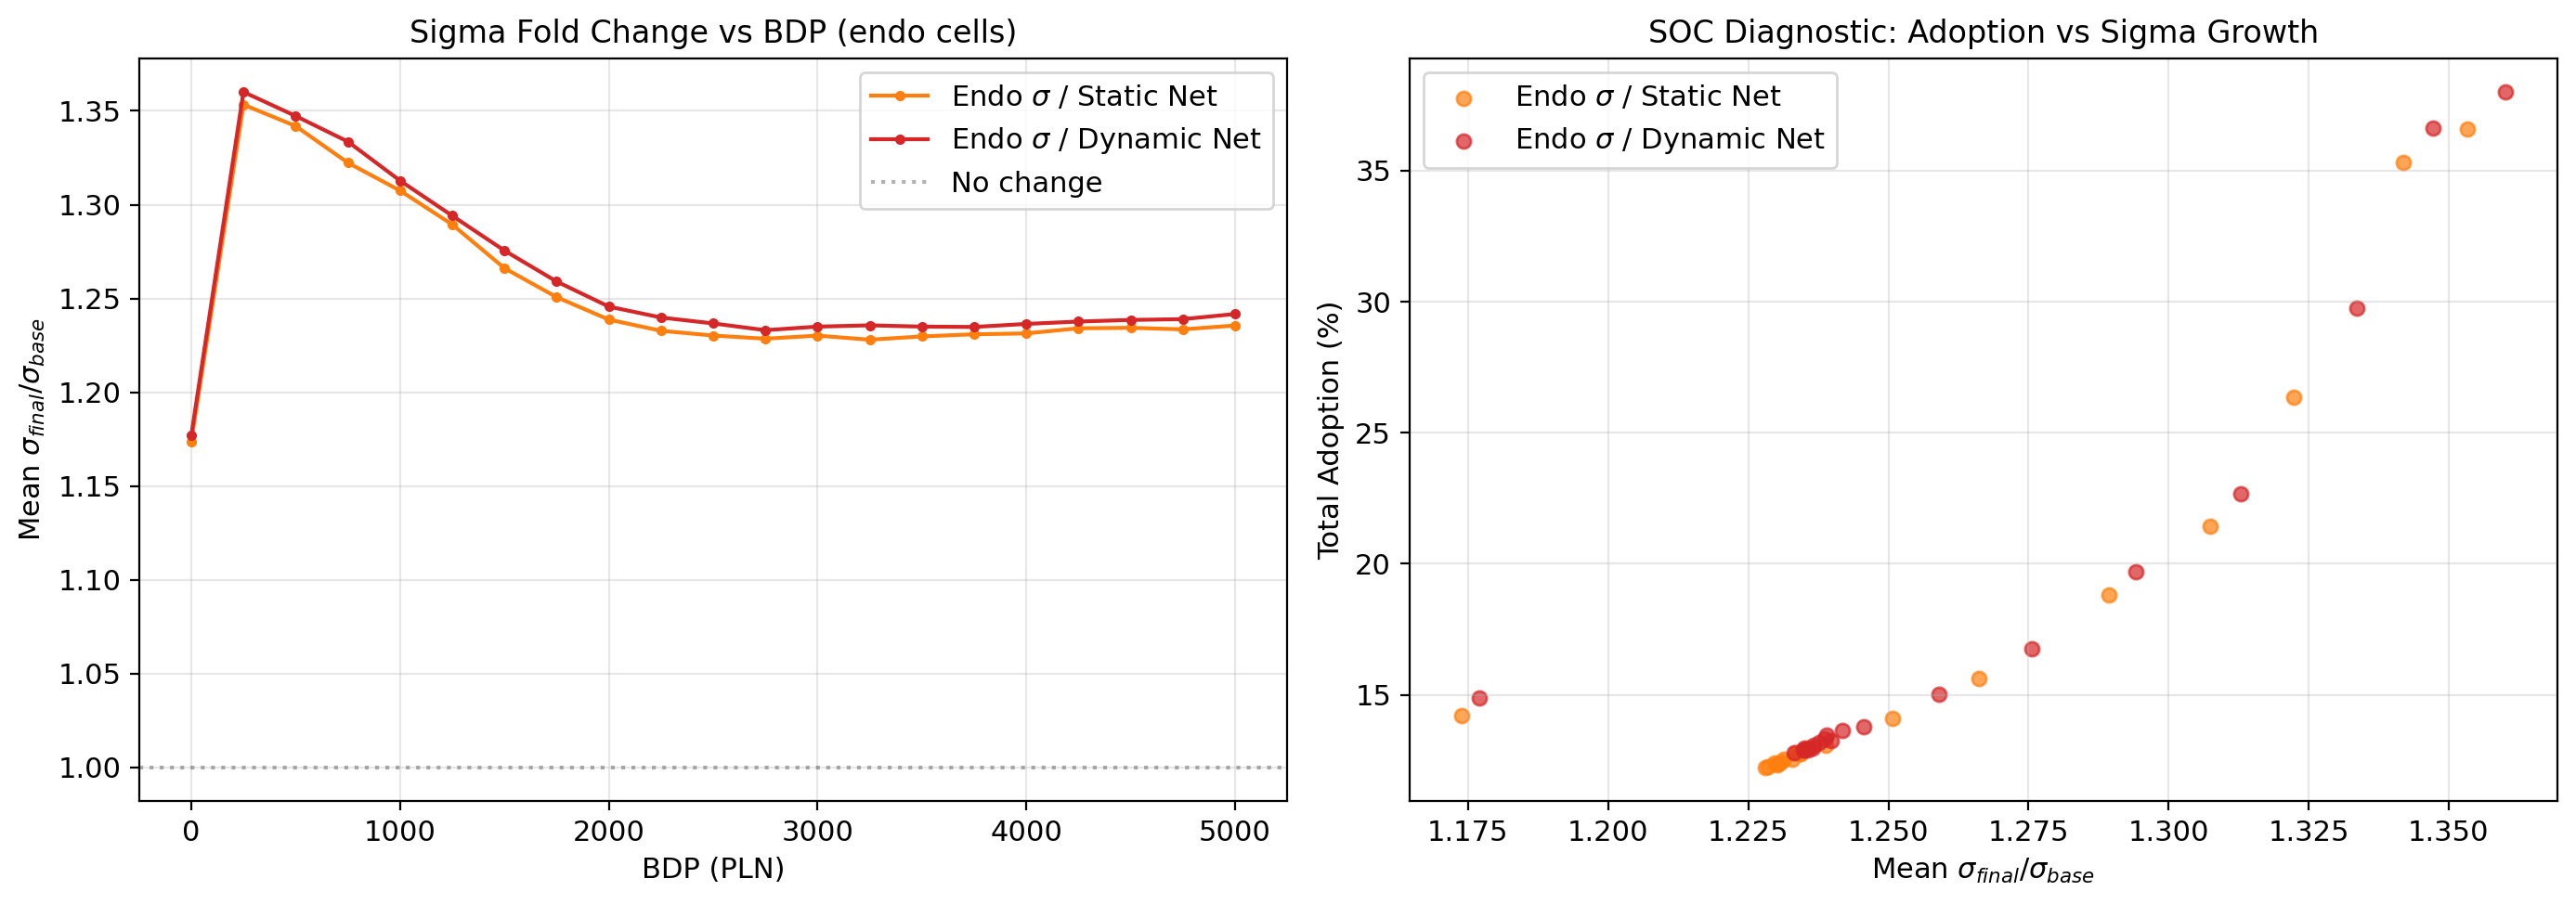
\includegraphics[width=0.85\textwidth]{../figures/fig12_soc_diagnostic.png}
    \caption{SOC diagnostic. Left: mean $\sigma$ fold change vs.\
    BDP for endogenous cells. Right: adoption vs.\ $\sigma$ fold change
    (scatter across BDP levels). The positive correlation reflects the
    learning feedback loop, not self-organized criticality.}
    \label{fig:soc}
\end{figure}

We therefore conclude that endogenous $\sigma$ evolution does
\emph{not} produce SOC in this model. The system does not self-tune
to the critical point; instead, it exhibits a positive feedback loop
where adoption and $\sigma$ growth reinforce each other, amplifying
the transition near BDP$_c$ but not driving the system toward it.


%======================================================================
\section{Discussion}\label{sec:discussion}
%======================================================================

%----------------------------------------------------------------------
\subsection{Robustness of Universality}\label{sec:robustness}
%----------------------------------------------------------------------

The central result of this paper is that the phase structure discovered
in Paper~IV is \emph{robust to endogenization}. Specifically:

\begin{enumerate}
  \item The reentrant (inverted-U) adoption shape survives in all
  four factorial cells and across all $\lambda$ and $\rho$ values
  tested. This shape---which implies an optimal BDP exists and that
  exceeding it is counterproductive---is the most policy-relevant
  feature of the model, and it is fully preserved.

  \item The critical point $\mathrm{BDP}_c$ shifts by at most one
  grid spacing (250~PLN, from 500 to 750) under dynamic rewiring
  or fast learning. Given the 250~PLN grid resolution, this is the
  \emph{minimal detectable} shift. The true shift may be smaller.

  \item The magnitude of the shift follows clear rules:
  $\lambda \le 0.02$ preserves $\mathrm{BDP}_c = 500$;
  $\lambda \ge 0.05$ shifts it to 750;
  $\rho \in [0.02, 0.1]$ shifts it to 750;
  $\rho \ge 0.2$ restores $\mathrm{BDP}_c = 500$.
\end{enumerate}

These findings extend the universality result of Paper~IV from
the exogenous to the endogenous domain. The phase transition is
not an artifact of static parameterization---it reflects a genuine
structural feature of the model economy.

%----------------------------------------------------------------------
\subsection{The Superadditivity Effect}\label{sec:superadd}
%----------------------------------------------------------------------

The +6.5~pp peak adoption boost in the full endogenous cell (vs.\
baseline) exceeds what either mechanism achieves alone. This
superadditivity arises because the two mechanisms operate on
complementary channels: endogenous $\sigma$ lowers the adoption
threshold (making marginal firms more likely to automate), while
dynamic rewiring creates preferential hubs that amplify contagion
(making adoption spread faster once it starts). The combination
produces a stronger positive feedback loop than either channel
alone.

From a policy perspective, the superadditivity implies that
economies experiencing both rapid learning and network restructuring
(e.g., emerging digital ecosystems) will exhibit more pronounced
adoption dynamics than models with static technology or networks
would predict. The optimal BDP must account for these amplification
effects.

%----------------------------------------------------------------------
\subsection{Why Not SOC?}\label{sec:why_not_soc}
%----------------------------------------------------------------------

The absence of self-organized criticality is informative. In canonical
SOC systems (sandpile models, forest fires), the dynamics
\emph{dissipate} energy or material at the boundary, creating a
natural mechanism for the system to hover near criticality
\parencite{Bak1996}. In our model, $\sigma$ evolution is a
\emph{positive} feedback: adoption raises $\sigma$, which lowers
the threshold, which raises adoption. This is an amplifying loop,
not a dissipative one. The ratchet constraint (Equation~\ref{eq:sigma_dynamics}) further prevents the oscillatory dynamics
that SOC requires.

For SOC to emerge in this class of models, one would need a
\emph{negative} feedback channel---for example, resource depletion,
skill obsolescence, or market saturation that reduces $\sigma$ when
adoption is too high. The purely increasing-returns specification
used here is insufficient.

%----------------------------------------------------------------------
\subsection{The Non-Monotonic $\rho$ Effect}\label{sec:nonmono}
%----------------------------------------------------------------------

The non-monotonic dependence of $\mathrm{BDP}_c$ on $\rho$
(Figure~\ref{fig:bdpc_rho}) has an elegant interpretation in terms
of network science. At $\rho = 0$, the network is a static
Watts--Strogatz small world. At moderate $\rho$ (0.02--0.1),
preferential attachment generates scale-free-like hubs that concentrate
influence and shift the critical point. But at high $\rho$ ($\ge 0.2$),
the network refreshes so rapidly that any emergent structure is
immediately destroyed, and the effective topology reverts to a random
graph---which, as Paper~IV demonstrated, has the same $\mathrm{BDP}_c$
as the small-world network \parencite{Maciaszek2026d}.

This mirrors results from the statistical physics of networks, where
dynamic rewiring at intermediate rates can produce qualitatively
different behavior from both the static and fully-random limits
\parencite{Albert2002, Castellano2009}. The window $\rho \in [0.02,
0.1]$ defines a ``structured rewiring'' regime where preferential
attachment creates meaningful heterogeneity.

%----------------------------------------------------------------------
\subsection{Limitations}\label{sec:limitations}
%----------------------------------------------------------------------

Several limitations should be noted. First, the BDP grid spacing of
250~PLN limits our ability to precisely locate $\mathrm{BDP}_c$.
The observed shift from 500 to 750 is the minimal detectable change;
a finer grid might reveal a continuous drift rather than a discrete
jump. Second, the learning rule (Equation~\ref{eq:sigma_dynamics})
is deliberately simple---a single-parameter logistic growth with
ratchet. Richer specifications (e.g., sector-specific $\lambda$,
learning spillovers across sectors, or depreciation) could produce
different dynamics. Third, the dynamic network model replaces
bankrupt firms with homogeneous Traditional entrants; heterogeneous
entrants (varying technology levels) could alter the results.
Fourth, we study only the PLN monetary regime; the EUR regime with
SGP constraints may respond differently to endogenization.

%----------------------------------------------------------------------
\subsection{Policy Implications}\label{sec:policy}
%----------------------------------------------------------------------

The key policy message is reassuring: the optimal BDP identified in
Papers~I--II ($\sim$500~PLN) remains approximately correct even when
technology and networks evolve endogenously. Policymakers need not
fear that endogenous dynamics will qualitatively alter the
cost--benefit calculus of BDP. The quantitative effect is an
\emph{increase} in peak adoption of 5--7~pp under endogenous
dynamics, suggesting that static models may somewhat \emph{underestimate}
the scale of the automation transition, but the optimal intervention
point is essentially unchanged.

The sector stratification in $\sigma$ growth (Figure~\ref{fig:sigma_heatmap})
has a direct policy implication: sector-specific transition support
should be concentrated on the high-$\sigma$ sectors (BPO/SSC,
Manufacturing) where endogenous technology dynamics are strongest,
rather than spread uniformly. Low-$\sigma$ sectors (Public, Healthcare)
are largely unaffected by endogenous dynamics and do not require
additional policy attention beyond what the static model prescribes.


%======================================================================
\section{Conclusion}\label{sec:conclusion}
%======================================================================

This paper tested whether the universality of AI adoption phase
transitions---established in Paper~IV under static, exogenous
conditions---survives when both the technology parameter~$\sigma$
and the inter-firm network are made endogenous. Through a $2 \times 2$
factorial design with 10,080 Monte Carlo simulations, we find that
universality is \emph{perturbed but preserved}: the reentrant adoption
shape is fully robust across all factorial cells, the critical point
shifts by at most 250~PLN, and the effects of the two endogenous
mechanisms are superadditive. Endogenous $\sigma$ does not produce
self-organized criticality; instead, a positive feedback loop between
adoption and learning amplifies the transition without driving the
system to the critical point.

The accumulated evidence across five papers---spanning monetary regimes,
empirical calibration, network topology, decision rules, system size,
and now endogenous dynamics---establishes that the reentrant phase
transition at $\mathrm{BDP}_c \approx 500$~PLN is a fundamental
structural feature of the model economy, robust to every dimension
of variation we have tested.


%======================================================================
\printbibliography
%======================================================================

\end{document}
